%%%%%%%%%%%%%%%%%%%%%%%%%%%%%%%%%%%%%%%%

% SENSYN: Handguides
% Authors: Katharina Krüsselmann, Marcel Haas, Jim Achterberg, Marco Spruit, Marieke Liem
% Created: March 2024

%%%%%%%%%%%%%%%%%%%%%%%%%%%%%%%%%%%%%%%%

%%%%%%%%%%%%%%%%%%%%%%%%%%%%%%%%%%%%%%%%
% Document Class
%%%%%%%%%%%%%%%%%%%%%%%%%%%%%%%%%%%%%%%%

\documentclass[12pt, twoside]{book}   

%%%%%%%%%%%%%%%%%%%%%%%%%%%%%%%%%%%%%%%%
% Document Setup
%%%%%%%%%%%%%%%%%%%%%%%%%%%%%%%%%%%%%%%%
	
%%%%%%%%%%%%%%%%%%%%%%%%%%%%%%%%%%%%%%%%
% Document Setup
%%%%%%%%%%%%%%%%%%%%%%%%%%%%%%%%%%%%%%%%
	
\usepackage{geometry}                		
\geometry{a4paper}     
\usepackage{url}             
\usepackage{graphicx}
\usepackage{parskip}
\usepackage{amssymb}
\usepackage{enumitem}
\usepackage[
backend=biber,
style=numeric-comp,
sorting=none
]{biblatex}
\addbibresource{SENSYN_bib.bib}
\usepackage[
colorlinks=true,
citecolor=black,
linkcolor=black,
filecolor=magenta,
urlcolor=blue]{hyperref}
\usepackage{soul}
\usepackage{fancyhdr}
\usepackage{tikz}
\usetikzlibrary{calc}
\usepackage{setspace}
\usepackage[osf]{newtxtext}
\usepackage{background}
\usepackage{float}
\usepackage{listings}
\usepackage{xcolor}
\usepackage{subfigure}
\usepackage{booktabs}
\usepackage{orcidlink}
\usepackage{titlesec}
\usepackage{array}

% Set line spacing
\onehalfspacing

% Set space between paragraphs
\setlength{\parskip}{1em}

% Banner bottom
\backgroundsetup{
  scale=1,
  color=black,
  opacity=0.7, 
  angle=0,
  position=current page.south,
  vshift=20pt, 
  hshift=0pt,
  contents={
\includegraphics[width=\paperwidth]{Images/banner.png}}
}


% page numbers 
\fancypagestyle{plain}{
    \fancyhf{} % Clear all header and footer fields

    % Page number positioning
    \fancyfoot[LE]{\thepage} % Left side on even pages
    \fancyfoot[RO]{\thepage} % Right side on odd pages
    


    % Adjust the vertical positioning
    \renewcommand{\headrulewidth}{0pt} % Remove header line
    \renewcommand{\footrulewidth}{0pt} % Remove footer line
    \setlength{\footskip}{40pt} % Adjust as needed to avoid overlap with banner
}

%Settings for python code in document 
\lstset{
    language=Python,
    basicstyle=\ttfamily\footnotesize,  % Style for the code text
    keywordstyle=\color{blue},          % Style for Python keywords
    stringstyle=\color{green},          % Style for strings
    commentstyle=\color{gray},          % Style for comments
    showspaces=false,                   % Show spaces as underscores (usually false)
    showstringspaces=false,             % Don't show spaces in strings
    numberstyle=\tiny\color{gray},      % Style for line numbers
    numbersep=5pt,                      % Space between line numbers and code
    tabsize=4,                          % Tab size
    breaklines=true,                    % Automatic line breaking
    breakatwhitespace=false,            % Automatic line breaking only at whitespace
    frame=single,                       % Add a frame around the code
    captionpos=b,                       % Caption position
    numbers=left,                       % Line numbers on the left
    xleftmargin=2em,                    % Left margin
    framexleftmargin=1.5em              % Margin inside the frame
}


%%%%%%%%%%%%%%%%%%%%%%%%%%%%%%%%%%%%%%%%
% Document Info
%%%%%%%%%%%%%%%%%%%%%%%%%%%%%%%%%%%%%%%%

\title{Project SENSYN}
\author{Katharina Krüsselmann, Marcel Haas, Jim Achterberg, Marco Spruit, Marieke Liem}
\date{25 March 2024}	

%%%%%%%%%%%%%%%%%%%%%%%%%%%%%%%%%%%%%%%%
% Main Document
%%%%%%%%%%%%%%%%%%%%%%%%%%%%%%%%%%%%%%%%
					
\begin{document}
\pagestyle{plain}
\raggedbottom
%%%%%%%%%%%%%%%%%%%%%%%%%%%%%%%%%%%%%%%%
% Front Matter

\begin{titlepage}
    \thispagestyle{empty}
    \centering
    \vspace*{\fill}
    \Huge{Making Sensitive Data Open and Fair Through Synthetic Data Generation}\\
    \vspace{0.5cm}
    \Large{A guidebook}\\
   
    \vspace*{\fill}
    
    \begin{tikzpicture}[remember picture, overlay]
        \node at (current page.south) [anchor=south, inner sep=0] {
            
\includegraphics[width=\paperwidth, height=0.4\paperheight]{Images/cover.png}
        };
    \end{tikzpicture}
    
    \vspace*{\fill}
\end{titlepage}

\newpage
\thispagestyle{empty} % No headers or footers on this page

This guidebook is the final result of \href{https://www.nwo.nl/en/projects/osf231006}{Project SENSYN}, which is funded by the NWO Open Science Fund (Grant number OSF23.1.006). \\

\textbf{Authors} \\\\
Katharina Krüsselmann \orcidlink{0000-0001-6181-425X} \\
Institute of Security and Global Affairs, Leiden University \\

Jim Achterberg \orcidlink{0009-0000-9589-7831}  \\
Health Campus The Hague, Leiden University Medical Center \\

Dr. Marcel Haas \orcidlink{0000-0003-2581-8370} \\
Health Campus The Hague, Leiden University Medical Center \\

Prof.dr. Marco Spruit \orcidlink{0000-0002-9237-221X} \\
Institute of Advanced Computer Science, Leiden University \\
Public Health \& Primary Care, Leiden University Medical Center \\

Prof.dr. Marieke Liem \orcidlink{0000-0002-2653-4356} \\
Institute of Security and Global Affairs, Leiden University \\

August 2024

DOI: 10.5281/zenodo.13374277
\vspace*{\fill}

\newpage
\tableofcontents
    \thispagestyle{empty}

\cleardoublepage


%%%%%%%%%%%%%%%%%%%%%%%%%%%%%%%%%%%%%%%%
% Chapters

\chapter{Introduction: The promise of synthetic data for open science}
%%%%%%%%%%%%%%%%%%%%%%%%%%%%%%%%%%%%%%%%
% Introduction
%%%%%%%%%%%%%%%%%%%%%%%%%%%%%%%%%%%%%%%%


\label{introduction}

Open Science is a movement to promote and stimulate open and accessible research practices, not just at the stage of publishing research results, but throughout the research cycle as a whole: from preregistration of research ideas and processes, to open analysis protocols, open code, open data, open peer review, open access publications and all steps in between. These practices have the aim to make research more accessible and transparent, to foster collaboration, strengthen trust in research and increase the scientific and societal impact of research. This movement is gaining momentum globally, driven by the growing recognition of the value of open science to research for advancing knowledge and addressing societal challenges \cite{UNESCO}.

An integral part of every empirical research cycle is data, which, too, is part of open research practices. Open data and FAIR data are central to the ethos of open science. \textbf{Open data} refers to data that is freely available for anyone to use, reuse and redistribute, with as little restrictions as possible. \textbf{FAIR data}, on the other hand, emphasises that data should be \textbf{f}indable, \textbf{a}ccessible, \textbf{i}nteroperable, and \textbf{r}esuable. The concept of FAIR data was introduced to create an infrastructure around the reuse of scholarly data. While open data focuses on the unrestricted availability of data, FAIR data principles provide a framework for ensuring that data are not only accessible, but also well-organised, annotated, and structured in ways that make them useful and meaningful to researchers across disciplines. Thus, open and FAIR data are not synonyms: data can be open but not follow FAIR standards, whilst FAIR standards do not require data to be open without restrictions. Specifically, FAIR standards recognise that not all data can be made open and accessible to everyone at all times. Therefore, when it comes to open data, the principle "as open as possible, as restricted as necessary" is commonly applied, which contrasts the ideas of open data \cite{wilkinson2016fair}. 

Both open data practices and FAIR principles are associated with several benefits to researchers. By making data openly available, researchers can enhance the visibility and impact of their work, leading to increased citations and greater recognition within the scientific community. FAIR data practices improve data quality and facilitate data sharing and collaboration, enabling researchers to build on each other's work more effectively. This collaborative approach can lead to new insights, help to avoid duplication of data collection efforts, and accelerate the generation of new knowledge. Furthermore, open and FAIR data practices support transparency and reproducibility in research, which in return should enhance trust in the scientific process and results. In addition, more and more journals and funding agencies require researchers to share (meta)data or a justification for why data sharing is not possible. 

%%%%%%%%%%%%%%%%%%%%%%%%%%%%%%%%%%%%%%%%

\section{Hurdles for datasharing}

Despite these benefits, some researchers are reluctant to adopt open and FAIR data practices. There may be concerns about the misuse of data, loss of competitive advantage, and the potential for data to be misinterpreted or misrepresented when made openly accessible. Another concern about open and FAIR data sharing may relate to legal and ethical risks: The processing and sharing of personal data is protected under privacy regulations, such as the European General Data Protection Regulations (GDPR). The GDPR defines personal data as "any information relating to an identified or identifiable natural person ('data subject')" \cite{gdpr2016general}, which includes a wide range of information, from names and addresses to someone's gender or age, biometric data, and social identity markers. Some researchers may be faced with even more restrictive regulations, for example when working with highly sensitive data, such as crime-, financial- or health- data. In the face of these restrictions, researchers may opt out of sharing any part of their data.  

Yet, the consequences of a lack of data sharing cannot be understated, in particular in those disciplines that commonly work with sensitive and/or personal data. Pridemore, for example, notes a replication crisis in the field of criminology, which is partially brought about by the unwillingness of researchers to share their data and a lack of a culture that incentivises such practices, with potentially far-reaching consequences for crime and justice policies \cite{pridemore2018replication}. When it comes to societal impact of research, a lack of transparency may decrease trust in research and evidence-based policies \cite{freese2022advances,powers2019open}. 

In light of these and other issues resulting from a lack of sharing (sensitive) data, the question arises whether there are options to share data of personal and sensitive nature, whilst still protecting the privacy of research subjects and adhering to relevant regulations. With fast developments in artificial intelligence and machine learning  over the last few years, promising tools arose that offer new approaches of processing, and eventually sharing, data without violating privacy regulations. One of these tools is the concept of synthetic data, which is, in short, artificially manufactured data that mimics real data without referring to actual persons that are protected through GDPR and other regulations \cite{el2020practical,hradec2022multipurpose,jordon2022synthetic} (more on synthetic data in the next chapter). Although the idea of synthetic data has gained traction amongst statisticians, computer- and data-scientists and has been applied by some commercial and public organisations, it has not yet reached all academic disciplines (specifically in the social sciences and humanities). One main reason for the lack of attention on synthetic data in those fields is that the majority of discourse on synthetic data has focused on the underlying statistical and technical processes of data synthesis, rather than the application of synthetic data to various fields. In addition, existing literature on synthetic data is somewhat inaccessible as it requires advanced technical and statistical knowledge. As a result, researchers without the technical expertise to engage with existing literature may not be aware of options to making their personal data FAIR and open.


%%%%%%%%%%%%%%%%%%%%%%%%%%%%%%%%%%%%%%%%

\section{About this guidebook}
\label{intro:about}

This guide aims to introduce and stimulate the use of synthetic data as a promising tool to overcome obstacles to the sharing of sensitive data for public and research use, in particular to a non-technical audience. 
This guide includes a general introduction to the concept, possible applications, a non-technical explanation of the synthesis process, an introduction to open-source tools for data synthesis and an overview of how the privacy and utility of synthetic data needs to be evaluated.

\href{https://www.universiteitleiden.nl/en/research/research-projects/governance-and-global-affairs/project-sensyn#tab-1}{Researchers from Leiden University and the Leiden University Medical Centre} created this report in the context of Project SENSYN, which is funded through the \href{https://www.nwo.nl/onderzoeksprogrammas/open-science/open-science-fund}{NWO Open Science Fund}. More information on the project and its outputs can be found on the \href{https://osf.io/4gmjn/resources}{Open Science Framework project page} or the project's webpage \hl{ENTER HYPERLINK}.



\chapter{Synthetic data: an introduction}
%%%%%%%%%%%%%%%%%%%%%%%%%%%%%%%%%%%%%%%%
% Chapter 2: What is synthetic data
%%%%%%%%%%%%%%%%%%%%%%%%%%%%%%%%%%%%%%%%


\label{syntheticdata}

In short, synthetic data is artificially manufactured data. Synthetic data can encompass a wide range of data types, mirroring the diversity found in real-world datasets. It can be used for both structured data, such as tabular data where rows represent individual records and columns represent attributes, and unstructured data such as text, images, and audio. Examples of synthetic tabular data are health records, customer information, transaction records, and clinical trial data \cite{el2020practical,yan2022multifaceted,hradec2022multipurpose}. In terms of unstructured synthetic data common examples are chat logs, emails, social media posts and clinical notes for text \cite{sagduyu2018synthetic,li2021synthetic}, and medical scans and deepfakes for images \cite{patel2023deepfake,paproki2024synthetic}. 

Two main types of synthetic data can be differentiated: synthetic data that is created from scratch and not based on a particular real-world dataset, and synthetic data that is generated to mimic a (complete or partial) real-world dataset. 

\section{Creating synthetic data from scratch}
Synthetic data generated from scratch is entirely artificial and created without using any real-world data as a template. This type of synthetic data is constructed using mathematical models and algorithms that define specific characteristics of the data. For instance, researchers can use simulation techniques to generate datasets based on theoretical distributions and hypothetical scenarios, or their own domain-specific knowledge. This approach is particularly useful for testing hypotheses, developing algorithms, and conducting simulations where real-world data is either unavailable or unsuitable. Because it is not derived from actual data, synthetic data from scratch poses very little risk of compromising privacy \cite{el2020practical,soltana2017synthetic}. 

\vspace{5pt}
\begin{figure}[h!]
    \centering
    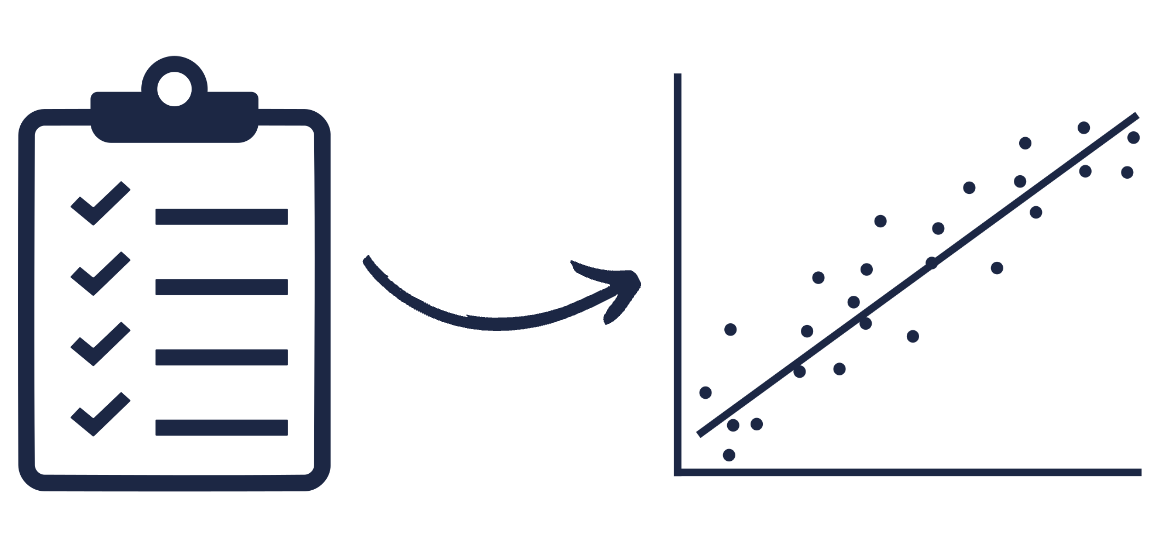
\includegraphics[width=0.5\textwidth]{Images/SyntheticData_1.png}
    \caption{Synthetic data from scratch.}
    \label{fig:sample_image}
\end{figure}
\vspace{5pt}

\section{Creating synthetic data based on real-world data}
Synthetic data designed to mimic-real-world data, on the other hand, is generated using real datasets as a basis. Advanced algorithms, including machine learning and deep learning techniques, are employed to analyse the patterns and relationships within the real data. These patterns are then used to generate synthetic data that closely mirrors the statistical properties and structure of the original dataset. The goal is to produce synthetic data that is realistic enough to be used in place of actual data for analysis, testing, training, or informative purposes while ensuring that no individual's personal information is exposed. This type of synthetic data is particularly valuable in fields like healthcare, finance, criminology or other social sciences, where data privacy is paramount but the need for realistic data is critical for effective research and development \cite{arnold2020really, jordon2022synthetic}. \\

\vspace{10pt}
\begin{figure}[H]
    \centering
    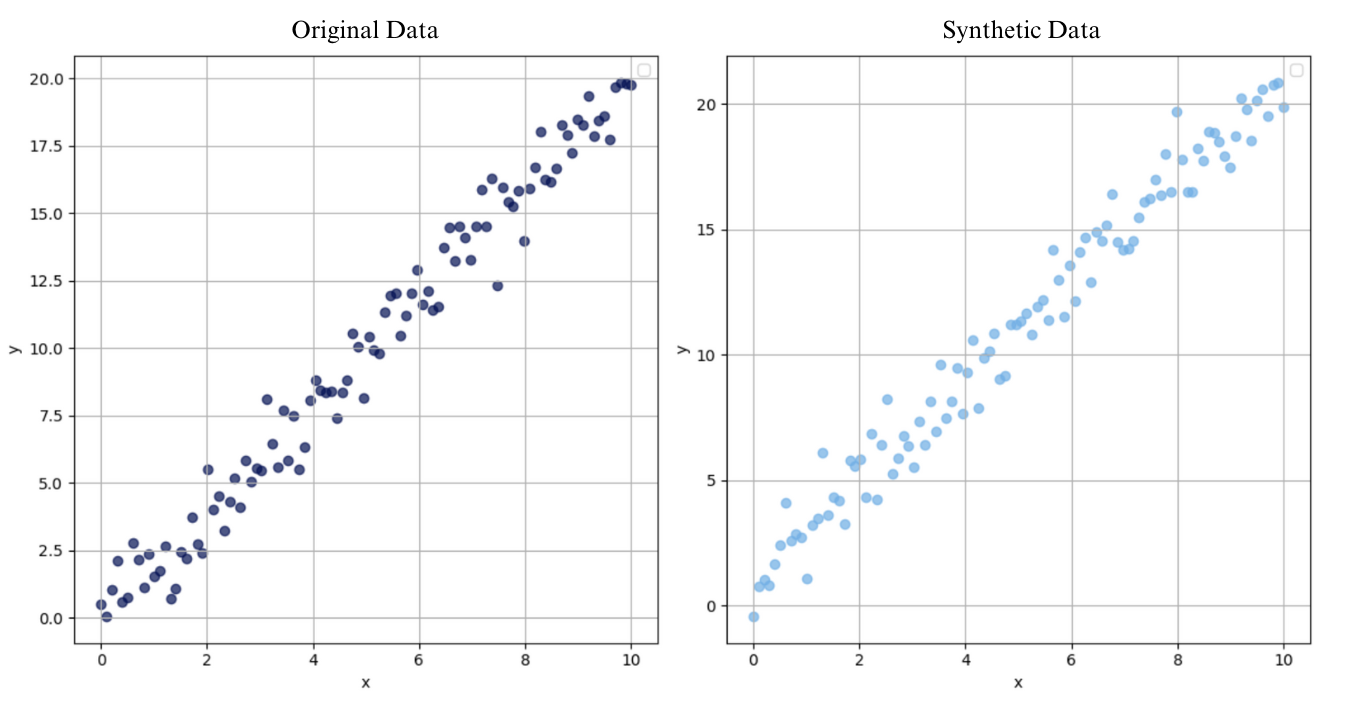
\includegraphics[width=\textwidth]{Images/Screenshot 2024-08-06 at 12.32.53.png}
    \caption{Synthetic data mimicking real-world data.}
    \label{fig:synthesis_2}
\end{figure} 
\vspace{10pt}


By understanding and utilising these two types of synthetic data, researchers can overcome many of the challenges associated with data privacy and sharing. Synthetic data from scratch provides a risk-free environment for preliminary research and hypothesis testing, while synthetic data that mimics real-world data enable researchers to perform realistic and meaningful analyses without compromising the privacy of individuals. Together, these approaches offer solutions for enhancing data sharing and collaboration in compliance with privacy regulations. 

\section{Advantages and disadvantages of synthetic data}

Synthetic data both provides significant benefits, whilst also presenting unique challenges. This section summarises some of the main advantages and disadvantages of synthetic data. Some of these are discussed more in-depth in the following chapters.

\textbf{Benefit: Privacy preservation}\\
Synthetic data can be generated without compromising sensitive information, making it an excellent tool for privacy-preserving data analysis. This is particularly relevant for fields that work with sensitive data, such as healthcare data, financial data or crime data, where data privacy regulations like GDPR and HIPAA are stringent. By using synthetic data, organisations can share and analyse data without exposing personally identifiable information and harming someone's right to privacy. 

\textbf{Benefit: Data augmentation}\\
Synthetic data is invaluable for augmenting small datasets. In fields such as machine learning, large datasets are crucial for training robust models. Synthetic data can fill gaps, balance class distributions, and enhance the diversity of training data, leading to improved model performance.

\textbf{Benefit: Cost-effective}\\
Generating synthetic data can be more cost-effective than collecting and labelling real-world data. Data collection processes can be expensive and time-consuming, often requiring significant human resources. Synthetic data, on the other hand, can be produced at a fraction of the cost and time.

\textbf{Benefit: Data- and environment manipulation}\\
Synthetic data allows for the creation of controlled environments where variables can be manipulated to study their effects. This is beneficial in scientific research and simulation studies, where researchers can systematically vary parameters and observe outcomes without real-world constraints.  

\textbf{Disadvantage: Quality concerns}\\
The quality of synthetic data depends heavily on the models used to generate it. Poorly designed synthetic data may not accurately reflect real-world patterns and correlations, leading to misleading conclusions and poorly performing machine learning models. So far, there are no standardised frameworks for quality control of synthetic data.

\textbf{Disadvantage: Potential biases}\\
If the models generating synthetic data are trained on biased real-world data, these biases can be perpetuated or even enhanced in the synthetic data. This can lead to biased outcomes in analyses and machine learning models, undermining the benefits of using synthetic data. 

\textbf{Disadvantage: Complexity of data generation}\\
Generating high-quality synthetic data can require advanced knowledge in data science, statistics, and domain-specific expertise for the evaluation of synthetic data. Developing and fine-tuning the synthesis process and associated models can be complex and time-consuming, requiring specialised skills and computational resources. Moreover, in many fields, there are no good examples yet of the generation and application of synthetic data.

\textbf{Disadvantage: Regulatory and ethical concerns}\\
While synthetic data can help navigate privacy regulations, it is not free from regulatory scrutiny. Misuse of synthetic data, especially when it comes to mimicking sensitive data, can raise ethical and legal issues. Furthermore, reliance on synthetic data must be carefully managed to avoid overestimating its reliability and validity, given possible quality control problems. 


\section{Potential uses for synthetic data in scientific research}

The potential of synthetic data for scientific research is plentiful, given its ability to replicate real-world data patterns while preserving privacy and circumventing data access limitations.

In \textbf{healthcare}, synthetic data plays a crucial role in medical research and clinical trials. Researchers can generate synthetic patient records that mimic real-world medical histories, allowing for the development and testing of new treatments and diagnostic tools without risking patient confidentiality. For example, synthetic data can simulate patient outcomes in clinical trials, providing a safe environment to asses the effectiveness and safety of new drugs before conducting actual trials. \cite{gonzales2023synthetic,arora2022generative,braddon2023exploring}

In \textbf{finance}, synthetic data is used to model financial markets and economic behaviour. Researchers can generate synthetic stock market data, transaction records, and costumer profiles to test trading algorithms and risk management strategies without exposing sensitive financial information. This approach not only safeguards privacy but also allows researchers to conduct extensive stress testing and scenario analysis, which is essential for understanding market dynamics and preparing for potential economic crises. \cite{assefa2020generating,eckerli2021generative}

\textbf{Environmental science} benefits from synthetic data through the simulation of environmental phenomena and the modelling of ecosystems. For instance, researchers can generate synthetic climate data to study the impacts of climate change under various scenarios. This include simulating temperature variations, precipitation patterns, and extreme weather events to predict their effects on ecosystems and human societies. Synthetic data also aids in the development of predictive models for natural disasters, such as floods and hurricanes, enhancing preparedness and response strategies. \cite{kravitz2021potential,perez2021machine}

In the fields of \textbf{criminology}, synthetic data is utilised to analyse crime patterns and develop predictive policing models. By creating synthetic crime reports and incident data, researchers can study trends and correlations without compromising the privacy of individuals involved in real criminal cases. This helps in identifying risk factors, improving law enforcement strategies, and designing more effective crime prevention programs. \cite{brunton2024using}

\textbf{Social sciences} also leverage synthetic data to study human behaviour and societal trends. Researchers can generate synthetic survey responses, demographic data, and social interactions to explore phenomena such as voting behavior, social mobility, and public opinion. This enables the examination of various hypotheses and policy impacts without the ethical and practical challenges associated with collecting real-world data. \cite{hradec2022multipurpose,kokosi2022overview}


\subsection{The use of synthetic data for open science practices}

Next to these practical applications, synthetic data offers several compelling advantages for open science practices and the FAIR principles. 

\textbf{Privacy preservation}\\ 
One of the most significant benefits of synthetic data is its ability to preserve privacy. Open science advocates for data sharing to foster transparency and reproducibility, but sharing real-world data often conflicts with privacy concerns, especially in sensitive fields like healthcare, medicine or social sciences. Synthetic data, which mimics real data without containing personal information, allows researcher to share datasets freely without risking breaches of confidentiality.

\textbf{Data accessibility}\\ 
Synthetic data facilitates broader access to data. Researchers can generate and share synthetic datasets that replicate the properties of restricted or proprietary data. This accessibility aligns with the FAIR principle of making data accessible, enabling a wider community of researcher to engage with and analyse the data, thus promoting inclusivity and collaboration. 

\textbf{Enhanced interoperability}\\
By using standardised methods and tools to generate synthetic data, researchers can ensure that datasets are compatible across different platforms and software. This interoperability is crucial for collaborative efforts where multiple teams might be using various systems and tools, allowing for seamless integration and analysis of data from diverse sources. 

\textbf{Reusability}\\
Synthetic data enhances the reusability of datasets. Because it can be shared without legal or ethical restrictions, synthetic data can be reused in multiple studies and by various research teams. This reusability supports the FAIR principle by maximising the utility of datasets, enabling continuous testing and validation of scientific hypotheses, and facilitating cumulative knowledge building. 

\textbf{Cost-effectiveness and efficiency}\\
Generating synthetic data can be more cost-effective and time-efficient than collecting new data. This efficiency allow researchers to quickly produce large, rich datasets necessary for robust scientific inquiry. Additionally, synthetic data can simulate rare or hypothetical scenarios, providing valuable insights that might be difficult or impossible to obtain from real-world data. \\

Overall, synthetic data significantly advances open science and the FAIR principles by enhancing privacy, accessibility, interoperability, and reusability. It empowers researchers to share and utilise data more freely and effectively, fostering a more collaborative and transparent scientific environment. 

\subsection{Synthetic data compared to other privacy-preserving methods}
The generation of synthetic data is not the first or only mechanism through which researchers can enhance and protect the privacy of their data. Other common mechanisms include anonymisation and differential privacy, yet both come with significant shortcomings.

\textbf{Anonymisation} involves removing or obfuscating personally identifiable information from dataset to prevent the identification of individuals. This method can be as easy as deleting attributes in a dataset that are related to personal information, such as names of individuals. As such, anonymisation is a widely used method. However, anonymisation has significant limitations, particularly in the face of advanced re-identification techniques. Even anonymised datasets can sometimes be linked with other data sources to re-identify individuals, compromising privacy. This limitation is especially pertinent in the era of big data, where vast amounts of auxiliary information are readily available \cite{majeed2020anonymization}. Additionally, obfuscating information which may be relevant may harm the overall utility of the dataset.

\textbf{Differential privacy} is another privacy-preserving mechanism \cite{dwork2006differential}. Differential privacy is a sophisticated technique that adds controlled noise to datasets, ensuring that the inclusion or exclusion of any single data point does not significantly affect the overall results. For example, noise can be added by altering certain values, such as salaries to obscure the exact, personal information. This method provides strong mathematical guarantees of privacy and is particularly effective in preventing re-identification. However, the added noise can degrade data utility, making it less useful for certain types of analyses. Implementing differential privacy also requires careful calibration to balance privacy and data quality, which can be complex and resource-intensive \cite{wasserman2010statistical,wood2018differential}. Additionally, it should be noted that differential-privacy can also be employed \textit{within} synthetic data generation, as a means to prevent re-identification from a synthetic dataset \cite{jordon2018pate,xin2022federated,sun2023generating}. \\


Each of these privacy-preserving methods comes with its own benefits and challenges. The choice of mechanism depends on the specific requirements and constraints of the research project.

\chapter{Synthesizing data: the process}
%%%%%%%%%%%%%%%%%%%%%%%%%%%%%%%%%%%%%%%%
% Chapter 3: Data synthesis
%%%%%%%%%%%%%%%%%%%%%%%%%%%%%%%%%%%%%%%%


Synthetic data generation is an iterative process that can be divided into three phases: the preparation phase, the data generation phase and the data evaluation phase. 

\vspace{10pt}
\begin{figure}[h!]
    \centering
    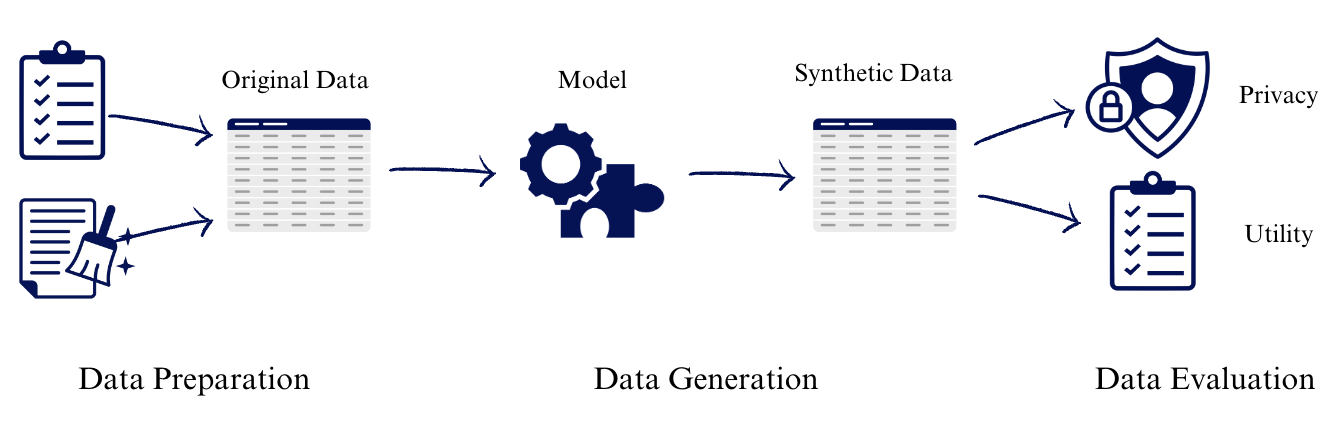
\includegraphics[width=\textwidth]{Images/Screenshot 2024-08-06 at 12.00.18.png}
    \caption{The Synthesis Process.}
    \label{fig:synthesis_1}
\end{figure}
\vspace{10pt}

\section{The preparation phase}

The goal of the preparation phase is to determine the ideal characteristics of the synthetic data and to choose a fitting generation method.

\textbf{Step 1a: When creating synthetic data from scratch: determine the structure and characteristics of the synthetic data} \\
Generating synthetic data from scratch requires meticulous preparation to ensure that the artificial data accurately reflects the intended use case and properties. The preparation phase involves several key steps. When developing synthetic data based on domain knowledge, deep comprehension of the domain is crucial. This includes understanding the key variables, their relationships, and the underlying processes governing the real-world data. For example, generating a synthetic database of a population of prisoners requires knowledge about the characteristics of prisoners. Equally, when the goal is to generate synthetic legal text, knowledge of legal jargon is a requirement. Another key step lies in defining the objectives for generating synthetic data. Will the data be used for testing algorithms, simulating specific scenarios, or conducting replication studies (to name just a few examples)? Depending on the answer to this question, the key features of the synthetic data need to be identified, such as their specific statistical properties: distributions, means, variances, correlations, and other relevant statistical metrics. For textual data, the desired length, complexity, tone or linguistic patterns need to be determined \cite{el2020practical,soltana2017synthetic}.

\textbf{Step 1b: When generating synthetic data to mimic real-world data: prepare the original dataset} \\
When generating synthetic data based on real-world data, it is still necessary to understand the key features of that data, such as distributions and relationships among variables for structured data, or patterns in language, sentiments, topic and structure for unstructured data, such as texts or audio. This knowledge is later required to evaluate the quality and usefulness of the synthetic dataset. In addition, data cleaning and preprocessing are crucial at this stage to ensure the quality and consistency of the real-world data, which serves as a benchmark for the synthetic data. Any mistakes, biases, outliers, special characteristics or irrelevant information need to be resolved or at least identified before the synthesis, as the synthesis process would mimic or even enhance those mistakes. Finally, any additional requirements for the synthetic data, such as logical rules, need to be determined. For example, if the original dataset contains a variable classifying individuals as either adult or minor, as well as a variable on the specific age of the individual, the model may recognise that individuals classified as minor have a significantly lower age than those classified as adults, but it may be necessary to create a rule that the specific age of minors in the synthetic dataset must not exceed 17. \\

\textbf{Step 2: Choosing the right generation method} \\
There are several methods to generate structured and unstructured synthetic data, and the choice depends on the type and complexity of the data, as well as the specific requirements of the project. Some of these methods may require advanced statistical knowledge, whilst others are more accessible to researchers without advanced expertise in statistics or data science. Some general categories of these methods are presented here.
 
\textbf{Rule based methods} for synthetic data generation rely on predefined rules, algorithms or simulations that mimic the behaviour and interactions found in real-world systems. These methods are particularly effective when no prior data is available, but domain knowledge is well-understood and can be explicitly encoded into the data generation process. In some disciplines, there may already be mathematical models that can be used for simulations, such as epidemiological models on the spread of diseases that can be used as a guidance for the synthetic data \cite{ajelli2018rapidd,gonzales2023synthetic}. Rule-based models are also suitable for demographic simulations, if demographic rules and census data offer enough information to create an artificial population. On the one hand, rule-based models can be highly tailored to specific domains, ensuring that synthetic data closely mimics real-world scenarios. Another benefit is that the rules through which the synthetic data is created need to be specified, which makes the data generation process transparent and understandable. On the other hand, it can be complex and time-consuming to create rule sets that accurately capture dynamic real-world behaviours. Additionally, synthetic data from rule-based methods can only include patterns and relationships which are known beforehand, thereby possibly excluding unknown but vital information. 

\textbf{Statistical models} use mathematical formulas to replicate the characteristics and relationships found in real data. For example, through random sampling, a model can generate synthetic data points from probability distributions that closely match the distributions observed in the real data. Thus, if the original data follows a normal distribution, synthetic data can be generated by sampling from a normal distribution with a similar mean and standard deviation as the original data. Other statistical models, such as copulas, may be more suited if one aims to model the dependency structure between multiple variables \cite{kamthe2021copula}. The vast variety of statistical models allows for flexible adaptation to different types of data and purposes for generating synthetic data. However, depending on the complexity of the original data, sophisticated statistical techniques and skills may be required to generate useful synthetic data. In addition, synthetic data generated through statistical models require a thorough validation to ensure that it accurately represent the real-world data \cite{pezoulas2024synthetic}. Also, statistical models often rely on strong assumptions regarding which distribution the data follows. These assumptions may not always hold true in practice. 

\textbf{Machine/Deep learning models} are used for generating more complex and realistic synthetic data. One example of a machine learning model are Generative Adversarial Networks (GANs). GANs involve two neural networks; one that generates synthetic data and one that evaluates it. They "compete" against each other, thereby improving the quality of the synthetic data over time \cite{wang2017generative}. Another example are Variational Autoencoders (VAEs), that learn to generate data by encoding the original data to grasp its key features and decoding these features into synthetic data points \cite{doersch2016tutorial,wan2017variational}. Bayesian networks require a map about the relationships between variables in the original data beforehand (e.g. based on expert knowledge), based on which they can learn about the probability that certain combination of features in the original data co-occur. This knowledge is then transferred into a synthetic dataset. These methods are powerful for creating high-fidelity synthetic data, but they require substantial computational resources and expertise and are thus not beginner-friendly. For textual data, language models such as GPT-3 are designed to generate and understand human language, such as grammar, syntax and semantics and replicate next text by predicting the next word or sequence of words \cite{li2023synthetic}. The benefit of machine learning models is their flexibility to learn and replicate complex patterns in data without heavily relying on assumptions, next to their ability to quickly scale to large datasets. However, compared to statistical and rule-based models, machine learning models are much more likely to replicate sensitive information in the synthetic data, due to over-fitting. In other words, these models may replicate the original data \textit{too} well. In addition, training these models can require (large amounts of) training data that the researchers needs to have available in addition to the data that needs to be replicated. Also, training and fine-tuning these machine models can require more advanced knowledge of computations.


%%%%%%%%%%%%%%%%%%%%%%%%%%%%%%%%%%%%%%%%

\section{The data generation phase}


\textbf{Step 3: Synthetic data generation} \\
The actual synthesis process is heavily dependent on the chosen model and the type of data that need to be synthesised. In general though, each of these models studies the real data or rules through which new synthetic data needs to be developed to determine the various patterns, relationships, and statistical properties within the original data or rules. 
Once the model has satisfactorily learned the properties of the real data, it can be utilized to generate new data points. This new data is not copied directly from the real data but is generated based on the patterns the model has learned, or rules that have been fed to the model. 

%%%%%%%%%%%%%%%%%%%%%%%%%%%%%%%%%%%%%%%%

\section{The data evaluation phase}

\textbf{Step 4: Evaluation of synthetic data} \\
Evaluation is a critical step in the process of generating synthetic data. When synthetic data is created from scratch, theory or domain knowledge, it needs to be evaluated against the rules and requirements set out at the beginning of the process. When synthetic data is generated to mimic real-world data, it needs to be evaluated on its similarity to the original data. When synthetic data is generated to ensure privacy, it needs to be evaluated and checked using controls for privacy. More detailed explanation on the evaluation of synthetic data is described in the following chapter. When the outcome of these evaluations does not align with the requirements for the synthetic data, the process of synthesising data needs to be repeated and adapted where necessary. As such, the synthesis of data becomes an iterative process.


\textbf{Optional: Further data anonymisation} \\
To ensure privacy, further steps may be taken to verify that the synthetic data does not contain any identifiable information. Even though synthetic data is inherently safeguarding personal information by generating artificial datapoints that do not relate to real-world persons, additional precautions can be implemented to safeguard against potential privacy risks. 


%%%%%%%%%%%%%%%%%%%%%%%%%%%%%%%%%%%%%%%%


\section{Open-source tools for synthetic data generation}

Synthetic data is not a new invention. Therefore, several open-source tools already exist that make the generation of synthetic data easier, due to their accessibility, flexibility, and the supportive communities that often accompany them. A few note-worthy open-source options are presented here, with a more comprehensive list in the appendix.

\textbf{Synthetic Data Vault} \\
The Synthetic Data Vault (SDV) is a comprehensive library that offers a variety of methods for generating synthetic data \cite{patki2016synthetic}. It supports generating tabular, sequential, and relational data. SDV utilises machine learning models to capture the distributions and relationships in the original data, ensuring realistic synthetic data generation. It is particularly useful for data scientists who need a robust, all-encompassing tool for different types of data. Next to synthetic data generation, it also incorporates various metrics for evaluating synthetic data quality. \textbf{Ease of use}: Moderate. SDV offers comprehensive documentation and examples, but understanding its full capabilities may require more extensive data science knowledge. \textbf{Programming language}: Python. 

\textbf{SynthCity} \\
SynthCity is a comprehensive library for synthetic data generation and evaluation \cite{qian2024synthcity}. It includes a wide variety of models for synthetic data generation, ranging from more classical machine learning algorithms, to Bayesian Networks, to advanced algorithms like GANs and VAEs. It includes methods for both tabular and imaging data generation. Furthermore, it contains a wide variety of metrics for comprehensive evaluation of synthetic data quality. \textbf{Ease of use}: Moderate. As in the SDV, SynthCity offers direct plug-and-play capabilities, but understanding its full potential may require more extensive data science knowledge. \textbf{Programming language}: Python. 

\textbf{YData} \\
YData Synthetic is an open-source tool that provides a user-friendly interface for generating synthetic data \cite{ydata}. It leverage GANs to create realistic data, focusing on enhancing the quality and diversity of synthetic datasets. \textbf{Ease of use}: YData Synthetic is designed to be easy to use, with straightforward interfaces and tutorials that make it accessible even for those with limited data science expertise. \textbf{Programming Language}: Python.

\textbf{Faker}\\
Faker is a lightweight library that generates fake data for various uses, including testing and development \cite{faker}. It can produce names, addresses, text, and other common data types. While not as advances as other tools for complex datasets, Faker is highly useful for quickly generating simple, structured synthetic data. \textbf{Ease of use}: High. Faker is extremely easy to use, with simple commands to generate various types of fake data quickly. \textbf{Programming Language}: Python. 

\textbf{Synthpop} \\
Synthpop is an R package focused on generating synthetic versions of data sets for statistical disclosure control \cite{nowok2016synthpop}. It is particularly popular in social science research, where it helps in creating synthetic datasets that preserve the statistical properties of the original data while protecting privacy. It relies on decision trees to sequentially populate synthetic features, to ultimately generate a synthetic dataset. \textbf{Ease of use}: Moderate. Synthpop provides extensive documentation, but some familiarity with statistical concepts and R programming is necessary. \textbf{Programming Language}: R (Python wrapper also available). 


\chapter{Privacy and utility of synthetic data}
%%%%%%%%%%%%%%%%%%%%%%%%%%%%%%%%%%%%%%%%
% Chapter 4: Data Evaluation
%%%%%%%%%%%%%%%%%%%%%%%%%%%%%%%%%%%%%%%%



\section{Privacy of synthetic data}

Ensuring the privacy of synthetic data is crucial for protecting individuals' sensitive information whilst allowing for useful data analysis.

\subsection{Privacy risks}

In general, we can distinguish between three different privacy risks:

\textbf{Re-identification risk} \\
Re-identification risk refers to the probability that an individual's identity can be discovered by matching anonymised or synthetic data back to the original dataset \cite{ochoa2001reidentification,el2008protecting}. This risk is a major concern in data privacy, particularly when sharing datasets containing sensitive information. Even if direct identifiers such as names and addresses are removed, individuals can often be re-identified through quasi-identifiers - attributes like age, gender, and zip code - when combined with other accessible datasources. 

\vspace{10pt}
\begin{figure}[H]
    \centering
    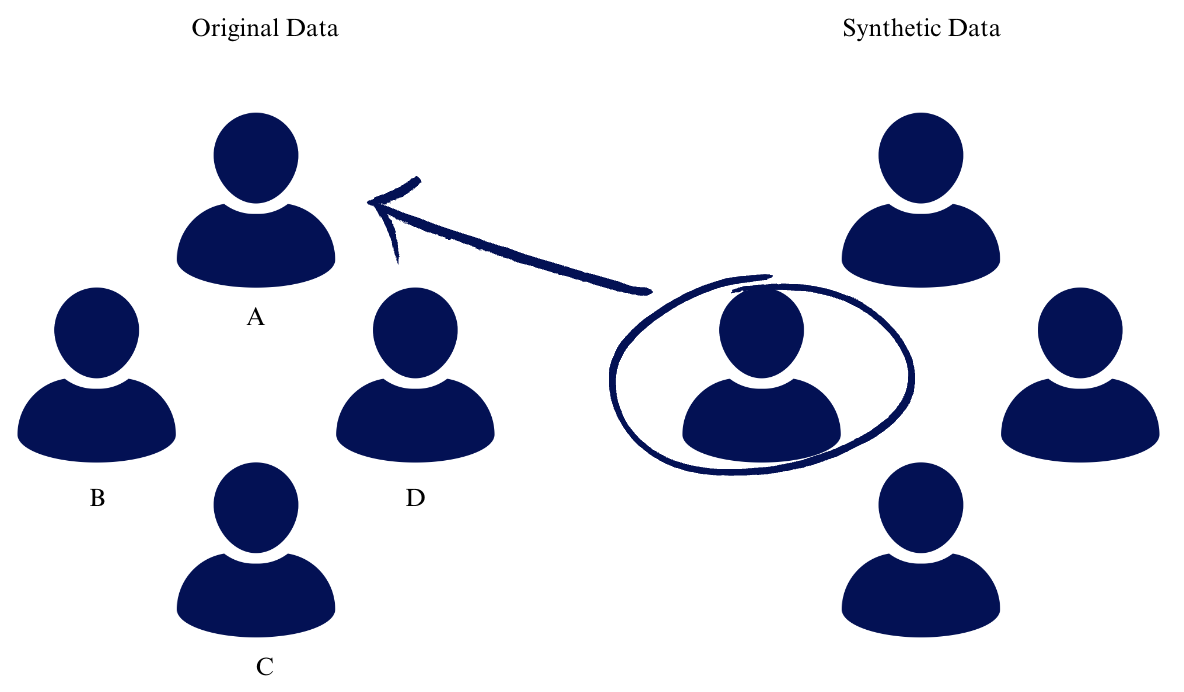
\includegraphics[width=0.5\textwidth]{Images/Reidentificationrisk.png}
    \caption{Re-identification risk}
    \label{fig:synthesis_1}
\end{figure}
\vspace{10pt}

\textbf{Membership inference risk} \\
Membership inference risk refers to the probability that an attacker can determine whether a specific individual's data was included in a dataset used to train a machine learning model or generate synthetic data \cite{hyeong2022empirical}. Such knowledge could reveal sensitive information about individuals, even if the data itself is anonymised. Understanding and mitigating this risk is essential for ensuring privacy in data sharing and open science practices.

\vspace{10pt}
\begin{figure}[H]
    \centering
    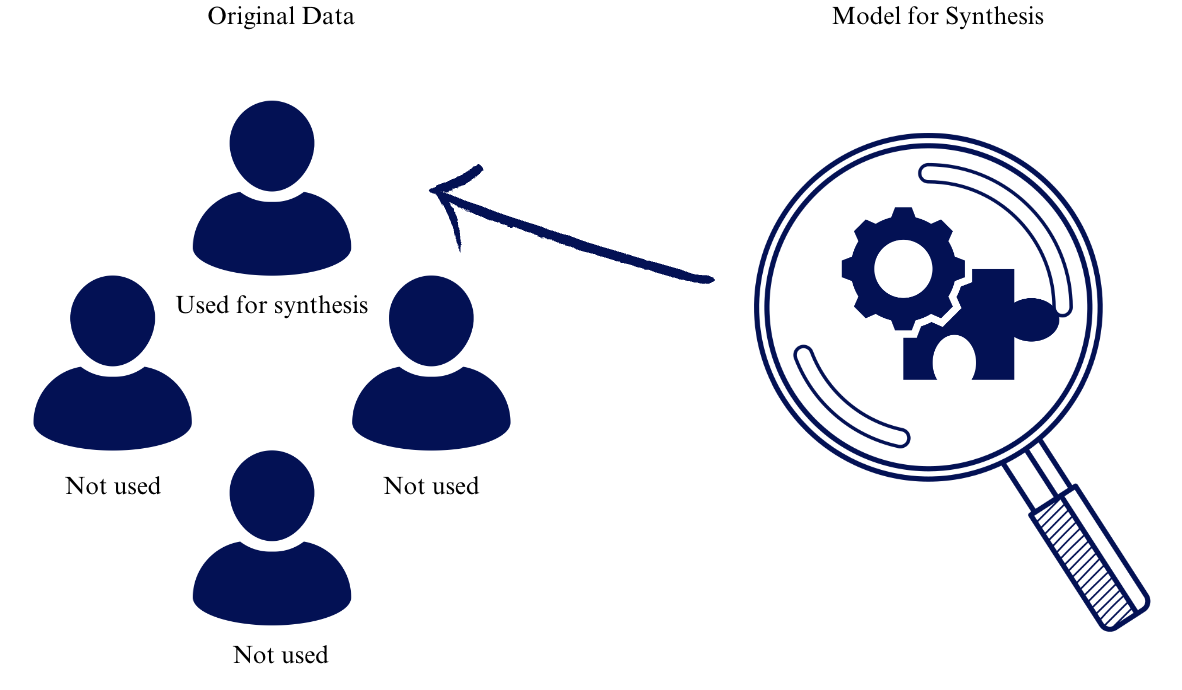
\includegraphics[width=0.5\textwidth]{Images/membershipinference.png}
    \caption{Membership inference risk}
    \label{fig:synthesis_1}
\end{figure}
\vspace{10pt}

\textbf{Attribute disclosure risk}\\
Attribute disclosure risk pertains to the likelihood that sensitive or private information about individuals can be inferred from a dataset, even if direct identifiers are removed. This risk arises when the remaining attributes in the dataset allow an observer to deduce specific details about individuals \cite{hittmeir2020baseline}. For instance, if a dataset includes a combination of age, zip code, and occupation, it might still reveal sensitive information about individuals, such as their income or health status. As such, attribute disclosure risk is similar to the re-identification risk. Yet, whereas the re-identification risk focuses on identifying individuals from data, attribute disclosure risk focuses on revealing sensitive attributes in particular. 

\textbf{Testing for Privacy Risks}\\
For each of these risks, various methods exist on how to measure them. These methods range from manually comparing records from the original dataset with records from the synthetic dataset based on quasi-identifiers, or checking whether outliers in the synthetic dataset can be linked to outliers in the original dataset to statistically measuring risks and mitigating them. Statistical tests can compare the similarities and differences between both the synthetic and original dataset, for example by calculating statistical distance measures. Examples are Euclidean distance, which connects each record in the synthetic dataset with the most similar record of the original dataset \cite{hittmeir2019utility}, or Bayesian estimation methods \cite{hu2018bayesian}. Another common method for measuring these risks is to simulate attacks on the privacy of the synthetic dataset. In these scenarios, models are trained to act as adversaries that aim to gain sensitive information from the synthetic dataset. These models, controlled by the researchers, can help to identify weak points in the synthetic data and quantify potential privacy risks \cite{boudewijn2023privacy,van2023membership,hittmeir2020baseline}.

 \subsection{The issue: lack of standards for privacy}
 Although there are a multitude of methods and techniques to evaluate the privacy of a generated synthetic dataset, there are currently several challenges that need to be addressed. 
 
 \textbf{Individualised data generation processes} \\
 Each generation of synthetic data involves unique processes tailored to specific use cases, datasets, and goals. Consequently, the techniques and methods used for calculating privacy risks can vary widely. This variability means that there is no one-size-fits-all approach for assessing privacy, and each synthetic data generation scenario may require a distinct set of privacy evaluation methods. This individualised approach complicates efforts to compare and validate privacy measures across different studies and applications.
 
 \textbf{Absence of standardised risk thresholds} \\
Possibly due to the complexity and variety of synthetic data generation methods and use cases, there are currently no universally accepted standards for defining what constitutes \textit{high} risk or \textit{low} risk in the context of privacy measures. Different techniques for evaluating privacy, such as re-identification risk or membership inference risk, may use varying thresholds to categorise risk levels. This lack of standardised thresholds creates inconsistencies in privacy assessments, making it challenging to interpret results and apply them consistently across different research contexts. Another hurdle is the difference between quantitative measures of privacy risks compared to the evaluation of privacy officers, lawyers or other experts in the field, who may hold different standards for risk thresholds than statistical measures and whose standards may differ per organisation or individual. Thus, potentially conflicting legal, ethical, statistical and organisational thresholds for privacy may hinder data scientists or researchers to develop synthetic data that can be used and shared. 
 
 \textbf{Evolving nature of synthetic data generation} \\
 The field of synthetic data generation is rapidly advancing, with new methods and techniques continually emerging. As a result, established privacy evaluation methods may become outdated or less effective over time. This constant evolution complicates the development and maintenance of standard practices for privacy assessments, as researchers must continually adapt their approaches to keep pace with technological advancements and emerging privacy risks.

 \subsection{Increasing privacy through differential privacy}
 Differential privacy is a mathematical framework used to provide privacy guarantees when releasing information about a dataset. It ensures that the output of a synthetic dataset does not significantly change when any single individual's data is added or removed, thus protecting individual privacy. In this framework, privacy is measured through two parameters: $\epsilon$ (epsilon) and $\delta$ (delta). $\epsilon$ measures the privacy loss, whereas $\delta$ represents the probability of the privacy guarantee being violated. In practice, differential privacy can be applied by determining the desired levels of privacy based on the sensitivity of the data and the acceptable risk and applying the associated values for both $\epsilon$ and $\delta$. Depending on the chosen values for $\epsilon$ and $\delta$, noise is added to the synthetic dataset, meaning that random modifications are made to the data to obscure the contributions of individual data points. While differential privacy is a robust technique for protecting individual privacy in datasets, it has notable drawbacks, in particular in relation to the framework's complexity. Implementing differential privacy requires careful tuning of privacy parameters, which can be complex and context-dependent. This complexity can make it difficult for researchers without extensive expertise in privacy-preserving techniques to apply differential privacy effectively \cite{dwork2006differential}
 

\section{Utility of synthetic data}

Specifically in the context of open science, the utility of synthetic data is paramount, as it must not only preserve privacy but also effectively support research objectives. Utility measures are used to evaluate how well synthetic data replicates the original data's characteristics and supports scientific analysis. These measures ensure that while data privacy is maintained, the synthetic data remains valuable for the intended use cases. What constitutes \textit{valuable} may differ per use case and goal for the synthesis. The following measures are some of the most common utility measures:

\textbf{Statistical accuracy} \\
One of the primary utility measures is statistical accuracy, which assesses how well synthetic data reflects the statistical properties of the original dataset. This is often also called fidelity. Specifically, this means that synthetic datasets should accurately capture the distribution and relationships of key variables. Techniques such as the Kolmogorov-Smirnov test or Chi-Square, or simple visualisations, can be used to test and compare distributions between synthetic and real datasets, ensuring that synthetic data replicates these characteristics accurately. Correlation coefficients, like Pearson's or Spearman's rank correlation, help verify that relationships between variables are preserved. Accurate statistical representation is crucial for ensuring that synthetic data can be used effectively in a wide variety of scientific research where data integrity is vital \cite{dankar2021fake,el2020seven,arnold2020really}.

\textbf{Utility in data analysis and decision-making} \\
Synthetic data should support meaningful analysis and visualisation. For example, replication studies with synthetic data of studies using the original data should generate the same general results \cite{braddon2023exploring}. Researchers can also apply clustering or classification models to synthetic data and compare the results with those obtained from real data. Consistent findings suggest that synthetic data is useful for generating insights and conducting robust scientific analysis. Furthermore, synthetic data should lead to valid and actionable conclusions, reinforcing its utility in practical application. Two problems with using these types of utility measures is that they are inherently use-case dependent and require the original data as a comparison. Thus, when synthetic data created for data analysis is shared and used by others, it may become less useful when not used for similar tasks.

\textbf{User experience and interpretability} \\
Finally, the ease of use and interpretability of synthetic data are essential utility measures. For open science, synthetic data must integrate smoothly into existing research workflows and tools. It should be formatted in a way that is compatible with FAIR standards.


\section{The trade-off between privacy and utility}

Specifically in the context of open science, researchers may generate synthetic data with the goal to create a dataset that both preserves the privacy of the original data, whilst also creating a synthetic dataset that strongly mimics the original data, to enhance utility for statistical analysis, informational purposes or other use cases. However, researchers have to take into account a potential trade-off between utility and privacy.

The core of the trade-off lies in the fact that increasing utility often comes at the cost of decreased privacy protection, and vice versa. Specifically, such a trade-off could appear if the model through which the synthetic data is generated is \textit{overfitting}, thus mimicking the original data so well that - by chance - one or more records in the synthetic dataset have the exact same characteristics as ones in the original data. Conversely, as privacy safeguards become more stringent, for example by adding noise to the synthetic dataset, the synthetic data may become less representative of the original data, leading to potential inaccuracies in research findings. Finding an optimal balance requires careful consideration of both privacy needs and objectives for the synthetic data. The acceptable level of privacy and utility may vary per use case and context. Ultimately, the goal is to achieve a synthesis of data that adequately protects privacy while still providing valuable insights and supporting robust scientific research. This balancing act is essential for advancing open science while ensuring that individual privacy remains protected. 

\begin{figure}[H]
    \centering
    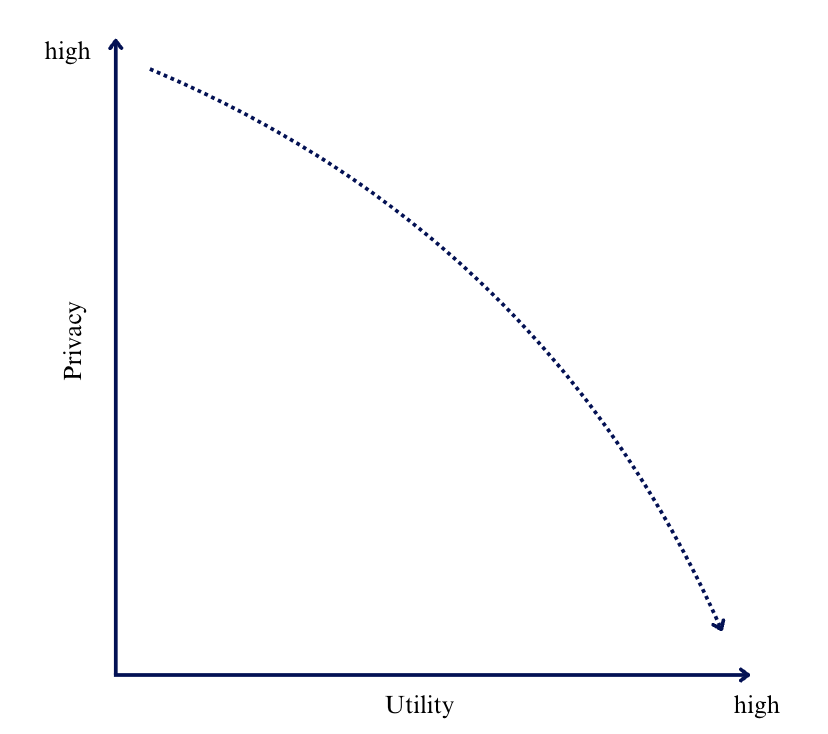
\includegraphics[width=0.8\textwidth]{Images/Screenshot 2024-08-06 at 13.06.13.png}
    \caption{Privacy-utility trade-off.}
    \label{fig:synthesis_1}
\end{figure}
















\chapter{Proof-of-concept: synthetic Dutch homicide data}
%%%%%%%%%%%%%%%%%%%%%%%%%%%%%%%%%%%%%%%%
% Chapter 5: Proof-of-concept: Synthetic Dutch Homicide Data
%%%%%%%%%%%%%%%%%%%%%%%%%%%%%%%%%%%%%%%%

\label{proofofconcept}

In order to showcase the applied use, advantages and limitations of synthetic data, this chapter will elaborate on the generation of a synthetic dataset based on the Dutch Homicide Monitor. This proof-of-concept covers the entire process of synthetic data generation (as described in Chapter 4), from data preprocessing and model selection to the generation and evaluation of synthetic data, using step-by-step discussions on the choices made during that process. 

\section{Dataset: The Dutch Homicide Monitor}

The Dutch Homicide Monitor is a dataset administered by researchers at Leiden University in the Netherlands (authors of this report). Through 25 nuclear attributes, the dataset captures detailed information on homicides committed in the Netherlands, including case-level information (such as the time of day and type of crime scene) as well as individual-level data of victims and (suspected) perpetrators, such as the age, gender, occupation and country of birth. The information included in the Dutch Homicide Monitor is derived from six sources: public sources, such as the annual homicide list collected by Elsevier Magazine, news articles and public court ruling, as well as non-public sources, such as police data, information from the public prosecution service and forensic records. As of June 2024, the Dutch Homicide Monitor captures all homicide committed between 1992 and 2023, which covers 5563 cases, and information on 5920 victims and 7542 (suspected) perpetrators \cite{DHM}. 

\textbf{Structure of the data}\\
The Dutch Homicide Monitor consists of 25 nucleus variables. Most of these variables (21) are categorical; only four variables (number of victims, number of perpetrators, age, date, description of incident) are non-categorical. Categories within a variable range from two (male/female) to 35 categories (victim-perpetrator relationship). In addition to these 25 variables, the dataset has three variables that act as identifying variables: a case number (which represents a case), a serial number (which represents each individual) and a variable that identifies one principal victim and perpetrator (if known) per case. These variables are defined in a \href{https://www.universiteitleiden.nl/binaries/content/assets/governance-and-global-affairs/isga/dfvm---coding-manual-marieke-liem.pdf}{coding manual}, which is shared with other researchers in the European Homicide Monitor network. 

\vspace{10pt}
\begin{table}[H]
\small
\centering
\begin{tabular}{@{}ll@{}}
\toprule
Case-level                  & Individual-level                 \\ \midrule
Case number                 & Serial number                    \\
Description                 & Crimescene                       \\
Number of victims           & Modus operandi                   \\
Number of perpetrators      & Type: victim or perpetrator?     \\
Spatial region              & Gender                           \\
City                        & Age                              \\
Year homicide was committed & Profession                       \\
Date of homicide            & Country of birth                 \\
Time of day                 & Alcohol (ab)use                  \\
                            & Drug (ab)use                     \\
                            & Violent history                  \\
                            & Context of homicide              \\
                            & Victim-perpetrator relationship  \\
                            & Main motive of perpetrator       \\
                            & Suicide (attempt) by perpetrator \\
                            & Stage in criminal justice system         \\ \bottomrule
\end{tabular}
\caption{Variables included in Dutch Homicide Monitor}
\label{tab:my-table}
\end{table}
\vspace{10pt}


The variables are embedded in the columns. Each record in that dataset represents an individual - either a victim or (suspected) perpetrator of the homicide. A variable 'Type' classifies the individual as either a victim or perpetrator. One homicide case can involve multiple victims and/or perpetrators, meaning that one case can span from two to six or even ten rows. Information stored on case-level variables is the same across the rows that belong to the same case, whereas individual-level information can vary for each row. A case number connects several rows (read: individuals) to the same case. 

\vspace{10pt}
\begin{table}[H]
\small
\centering
\begin{tabular}{@{}lllllll@{}}
\toprule
Case number & Serial number & Time of day & Type        & Gender & Age & .. \\ \midrule
1           & 1.1           & 6am-12pm    & Victim      & F      & 22  & .. \\
1           & 1.2           & 6am-12pm    & Perpetrator & M      & 24  & .. \\
2           & 2.1           & 6pm-12am    & Victim      & M      & 46  & .. \\
2           & 2.2           & 6pm-12am    & Perpetrator & M      & 55  & .. \\
2           & 2.3           & 6pm-12am    & Perpetrator & M      & 43  & .. \\ \bottomrule
\end{tabular}
\caption{Example of DHM structure}
\label{tab:my-table}
\end{table}
\vspace{10pt}

\subsection{Privacy of homicide data in the Dutch Homicide Monitor}
The Dutch Homicide Monitor contains sensitive personal information on victims and (suspected) perpetrators of homicide in the Netherlands. Being a victim or perpetrator of a (violent) crime in itself can be considered sensitive information. In addition, individual-level sensitive information includes the gender, age, country of birth, occupation, address of the incident and more. Although some of this information can be found in public sources, such as news articles, overall, this personal information is protected through the European Union's GDPR regulation, as well as agreements made with the Dutch National Police and Public Prosecution Office of the Netherlands on the handling of their data. The sensitive nature of the data limits the use of the Dutch Homicide Monitor: students, journalists or researchers who want to use the disaggregated dataset cannot immediately gain access. Researchers may apply to gain access to the dataset, yet this process can take up considerable time and efforts, making it infeasible for certain use cases. In addition, implementing FAIR standards to the dataset is limited, given that the dataset is neither accessible, interoperable, nor reusable. 

%%%%%%%%%%%%%%%%%%%%%%%%%%%%%%%%%%%%%%%%

\section{Generating a synthetic version of the Dutch Homicide Monitor}

\subsection{First attempt}

To begin with, we set a list of requirements for the to-be-generated synthetic dataset. We want a: 

\begin{enumerate}[label=\alph*)]
	\item fully synthetic dataset
	\item dataset with the same structure as the original data that allows for analysis on case-, victim- and perpetrator-level
	\item statistical accuracy that allows for replication of past studies using the original data
	\item safeguarding of sensitive information to adhere to GDPR and additional regulations associated with the original data
\end{enumerate}

Through these requirements, we aimed to generate a synthetic dataset that is complete and can be used for several purposes, such as student exercises, as a source of information for journalists and other stakeholders, as well as a source for future academic studies. In short, a dataset that can be registered and used for any possible future purpose.

\textbf{Step 1: Preparations} \\
Given that the requirements do not ask for much change to the original data, the preparations were minimal. As with any data analysis, we checked the data for internal inconsistencies, for accidental mistakes in the coding (e.g. 998 instead of 999), duplicates and so on.

Another concern during this phase was data quality. The fraction of missing data for certain cases can be high, e.g. due to a lot of missing information in the homicide, such as the identity of the perpetrator, or due to a lack of details in the available data sources. For example, police reports on earlier homicides may not have as much detail as police reports on more recent cases. In order to have a high-quality synthetic dataset of the Dutch Homicide Monitor, we decided to create a dataset that only contains ten years of high-quality homicide data.  After extracting these ten years of high-quality data from the Dutch Homicide Monitor, the new and to-be-synthesised dataset contained 1271 cases, and information on 1348 victims and 1711 (suspected) perpetrators. 

Finally, we determined two logical dependencies in our dataset that are present in the original data and would need to be replicated in a synthetic dataset. First, we determined that any homicide victim involved in a \textit{child homicide} needed to be \textit{younger than 17 years}. Another logical dependency in the original data is between the type of homicide and victim-perpetrator relationship. Specifically, we determined that homicides categorized as intimate partner homicides needed to co-occur with the victim-perpetrator relationship of \textit{partner} or \textit{ex-partner}.

\textbf{Step 2: Choosing generation method and tool} \\
The choice of generation method and tool was determined by two factors: First, the generation method needed to fit the structure of our data. Second, the generation method and tool specifically needed to be easy to use, as the goal of the project and this guide on synthetic data was to make synthetic data accessible to a broader audience without extensive knowledge of computations or data science. Therefore, we evaluated the extent of helpful and guiding documentation for each generation method and tool and selected a member of the project team with no experience with synthetic data as the lead for the generation process. Following the principals of open science, only open-source tools (thus no commercial options) were included in the decision process.

As mentioned in Section 3.1, three main categories of synthetic data generation methods can be distinguished: rule-based, statistical, and machine learning methods. We opted for a statistical method as rule-based methods are time-consuming to develop and rely heavily on prior domain knowledge, and our dataset is relatively small to justify using advanced machine learning methods like GANs and VAEs. An additional benefit of statistical methods over machine learning methods are increased interpretability of the generation process. To generate high-utility synthetic data, the statistical method should not only capture univariate distributions, but also dependencies between variables. An apt statistical method are thus copula models, which separately model univariate distributions and the dependency structure between variables, after which they are linked together to model the multivariate dataset \cite{nelsen2006introduction}.

Several tools use copulas as a basis for the synthesis of data. Yet, the structure of our data limited the options of tools available to us, given that not all tools are equipped to synthesise data with dependencies across rows and columns. After reviewing several options, we decided that the best approach to keep these dependencies would be through a multi-table synthesis. In this process, several tables linked through a common identifier are synthesised whilst keeping the relationships between the tables and variables. In order to prepare our data for this process, we divided the main dataset into three separate ones: one that includes four case-level variables, one that includes thirteen variables containing information on the victims and one that includes twelve variables related to information on the perpetrator. Some variables in the victim- and perpetrator-tables overlap, such as age, gender, country of birth or occupation. 

\vspace{10pt}
\begin{table}[h!]
\small
\centering
\begin{tabular}{@{}lll@{}}
\toprule
Case variables              & Victim variables                & Perpetrator variables            \\ \midrule
Case number                 & Serial number                   & Serial number                    \\
Description                 & Gender                          & Gender                           \\
Number of victims           & Age                             & Age                              \\
Number of perpetrators      & Profession                      & Profession                       \\
Spatial region              & Country of birth                & Country of birth                 \\
City                        & Alcohol (ab)use                 & Alcohol (ab)use                  \\
Year homicide was committed & Drug (ab)use                    & Drug (ab)use                     \\
Date of homicide            & Violent history                 & Violent history                  \\
Time of day                 & Crimescene                      & Main motive                      \\
                            & Modus operandi                  & Suicide (attempt) by perpetrator \\
                            & Context of homicide             & Stage in judicial system         \\
                            & Victim-perpetrator relationship &                                   \\ \bottomrule       
\end{tabular}
\caption{DHM variables split by related case-, victim- or perpetrator-level}
\label{tab:my-table}
\end{table}
\vspace{10pt}

The Synthetic Data Vault (SDV) is one of the very few open-source tools that allow for multi-table synthesis. In addition, it provides extensive documentation and support, which is why we chose the SDV for the synthesis of our homicide dataset. The SDV runs on Python and includes suggestions and requirements for data preparation for the synthesis of multi table data. Our data fulfilled most of the requirements, with the exception of a document/object that defines the meta data across the tables - in other words a document that provides information about the type of data, the identifier-variables that link the tables together and specific connections between the tables. This information can be set-up manually, following instructions in the SDV-documentation, but the SDV-package also comes with functions that can automatically detect this information from your tables, but these require additional verification and checks.

After following the required steps, our homicide dataset was split into one parent table (in our case, the table with case-level variables) and two child tables (one victim table, one perpetrator table). In this meta-data, the case number is identified as an id that connects the inter-dependent rows across those three tables. 
\vspace{10pt}
\begin{figure}[H]
    \centering
    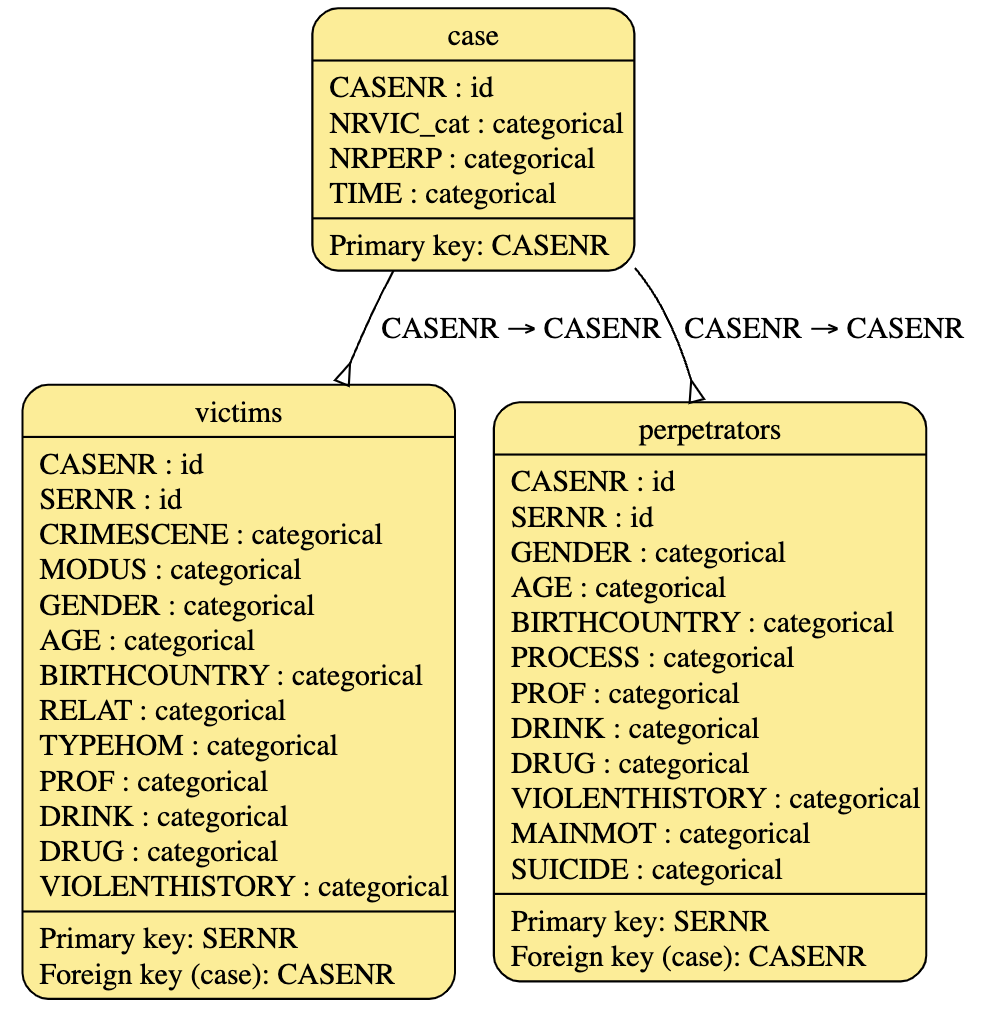
\includegraphics[width=0.6\textwidth]{Images/meta1.png}
    \caption{Dutch Homicide Monitor split into three separate datasets: cases, victims \& perpetrators}
    \label{fig:proof_1}
\end{figure}
\vspace{10pt}

In addition, we prepared the logical dependencies as identified in the preparation phase. Therefore, we wrote a code (available on \href{https://github.com/KKrusselmann/SENSYN}{Github}) that would force the model during the synthetic data generation to adhere to the rules set out about the dependency of child homicide and victim age, as well as between intimate partner homicide and victim-perpetrator relationship.

\textbf{Step 3: Generation of synthetic data} \\
The meta-data information prepared in the previous step is then used to create a synthesiser, that is an object that creates synthetic data. The meta-information provides the synthesiser with the relevant information about the structure of the original data, such as the number of columns or categories within a variable. This structure determines the desired structure of the synthetic dataset. After, we loaded the original data into this synthesiser through which it can learn about the patterns and relationships between the variables in our dataset. Finally, the synthesiser generates a synthetic dataset using the structure and identified relationships. We chose to generate as many cases as are included in the original dataset. \\

The result are three synthetic tables that together form the first synthetic version of the Dutch Homicide Monitor.

\vspace{10pt}
\begin{table}[]
\small
\begin{tabular}{@{}llll@{}}
\midrule
Case number   & Number of victims & Number of perpetrators & Time of day \\ \midrule
sdv-id-nFatwl & 1                 & 1                      & 6am-12am    \\
sdv-id-MulxVy & 1                 & 1                      & 12pm-6pm    \\
sdv-id-gzVJSQ & 2                 & 2                      & 12pm-6pm    \\
...           & ...               & ...                    & ...    \\ \bottomrule    
\end{tabular}
\caption{Synthetic case dataset (first three cases)}
\label{tab:my-table}
\end{table}
\vspace{5pt}

\begin{table}[]
\small
\begin{tabular}{@{}llllll@{}}
\toprule
Case number   & Serial number & Modus operandi              & Gender  & Age     & ... \\ \midrule
sdv-id-nFatwl & sdv-id-fgFyn  & Firearm                     & Missing & 65      & ... \\
sdv-id-MulxVy & sdv-id-MwbyTx & Missing                     & Missing & Missing & ... \\
sdv-id-gzVJSQ & sdv-id-cQNzXJ & Knife or other sharp object & Male    & Missing & ... \\
sdv-id-gzVJSQ & sdv-id-xgDRmZ & Knife or other sharp object & Missing & 24      & ... \\
...           & ...           & ...                         & ...     & ...     & ... \\ \bottomrule
\end{tabular}
\caption{Synthetic victim dataset (associated with first three cases)}
\label{tab:my-table}
\end{table}

\vspace{5pt}
\begin{table}[]
\small
\begin{tabular}{@{}llllll@{}}
\toprule
Case number   & Serial number & Gender & Age & Country of birth & ... \\ \midrule
sdv-id-nFatwl & sdv-id-Edlwqz & Male   & 19  & Missing          & ... \\
sdv-id-MulxVy & sdv-id-LWxGTc & Male   & 17  & Missing          & ... \\
sdv-id-gzVJSQ & sdv-id-imlpGf & Male   & 38  & Netherlands      & ... \\
sdv-id-gzVJSQ & sdv-id-UlNuoi & Male   & 24  & Netherlands      & ... \\
...           & ...           & ...    & ... &                  & ... \\ \bottomrule
\end{tabular}
\caption{Synthetic perpetrator dataset (first three cases)}
\label{tab:my-table}
\end{table}
\vspace{10pt}

\textbf{Step 4: Privacy and Utility Evaluation} \\ 
With regards to the utility, the generated synthetic dataset was of moderate quality.
The SDV package offers several options within the package to evaluate the quality of the synthetic data. First, one can run diagnostics on the synthetic data structure and validity, which test whether the synthesiser adhered to the categories of the original dataset, that variables classified as id have unique numbers for each row and that all of the variables have been adapted into the synthetic dataset. In our synthetic dataset, both statistics were at 100 percent, meaning that the structure and validity of the original dataset was fully adopted onto the synthetic dataset.

Secondly, SDV can create a quality report of the synthetic dataset that measures the similarity of the synthetic dataset to the original dataset, based on a comparison of the univariate and bivariate distributions in the synthetic and original dataset. In this attempt, the scores for the univariate distributiom measure was 79.17\%, and the measure for bivariate distributions 57.21\%, as shown in the table below. Additional reports show that some variables had a significantly lower score than others.

\vspace{10pt}
\begin{table}[H]
\small
\resizebox{\textwidth}{!}{
\begin{tabular}{@{}lll@{}}
\toprule
Quality Type &
  Score (\%) &
  Interpretation \\ \midrule
Data validity &
  100 &
  \begin{tabular}[c]{@{}l@{}}The synthetic data has the same internal structure \\ as the original one\end{tabular} \\
Data structure &
  100 &
  \begin{tabular}[c]{@{}l@{}}The synthetic data has the same columns \\ with the same names\end{tabular} \\
Relationship validity &
  99.94 &
  \begin{tabular}[c]{@{}l@{}}Each case in the victim \& perpetrator datasets \\ are linked to a case in the case dataset\end{tabular} \\
Univariate distribution &
  79.17 &
  \begin{tabular}[c]{@{}l@{}}A variable in the synthetic dataset is on average \\ 80\% similar to the variable in the real dataset\end{tabular} \\
Bivariate distribution within one table &
  57.21 &
  \begin{tabular}[c]{@{}l@{}}The relationship between two variables in the \\ synthetic data is about 57\% similar to the \\ relationship in the real dataset\end{tabular} \\
Structure across tables &
  94.98 &
  \begin{tabular}[c]{@{}l@{}}Almost each case in the synthetic dataset has the \\ same number of victims and perpetrators associated \\ as in the real dataset\end{tabular} \\
Bivariate distribution across tables &
  79.91 &
  \begin{tabular}[c]{@{}l@{}}The relationship between two variables across \\ the three synthetic datasets is about 80\% similar \\ to the relationship in the real data\end{tabular} \\
Overall &
  75.82 &
  \begin{tabular}[c]{@{}l@{}}Overall, the synthetic dataset compares \\ around 75\% to the real data\end{tabular} \\ \bottomrule
\end{tabular}
}
\caption{General quality report}
\label{tab:my-table}
\end{table}
\vspace{10pt}

\vspace{10pt}
\begin{table}[H]
\small
\centering
\begin{tabular}{@{}ll@{}}
\toprule
Variable                                              & Score (\%)   \\ \midrule
Perpetrator's main motive                             & 90.54 \\
Perpetrator committed or attempted suicide            & 89.61 \\
Perpetrator drug (ab)use                              & 88.8  \\
Perpetrator gender                                    & 84.74 \\
Perpetrator birth country                             & 83.58 \\
Perpetrator violent history                           & 82.77 \\
Perpetrator profession                                & 81.61 \\
Perpetrator age                                       & 81.61 \\
Perpetrator alcohol (ab)use                           & 30.16 \\
Status of case against perpetrator in judicial system & 30.1 \\ \bottomrule
\end{tabular}
\caption{Example: quality of each variable in the synthetic perpetrator dataset, ranked from highest to lowest similarity score}
\label{tab:my-table}
\end{table}
\vspace{10pt}

The varying degrees of quality across the synthesised variables are also visible in visualisations that compare the univariate and bivariate distributions of the synthetic and original dataset. Through these visualisations, we determined that about 70 percent of the variables in the synthetic dataset compared well to the original data, such as the time of day the homicide was committed.

\vspace{10pt}
\begin{figure}[H]
    \centering
    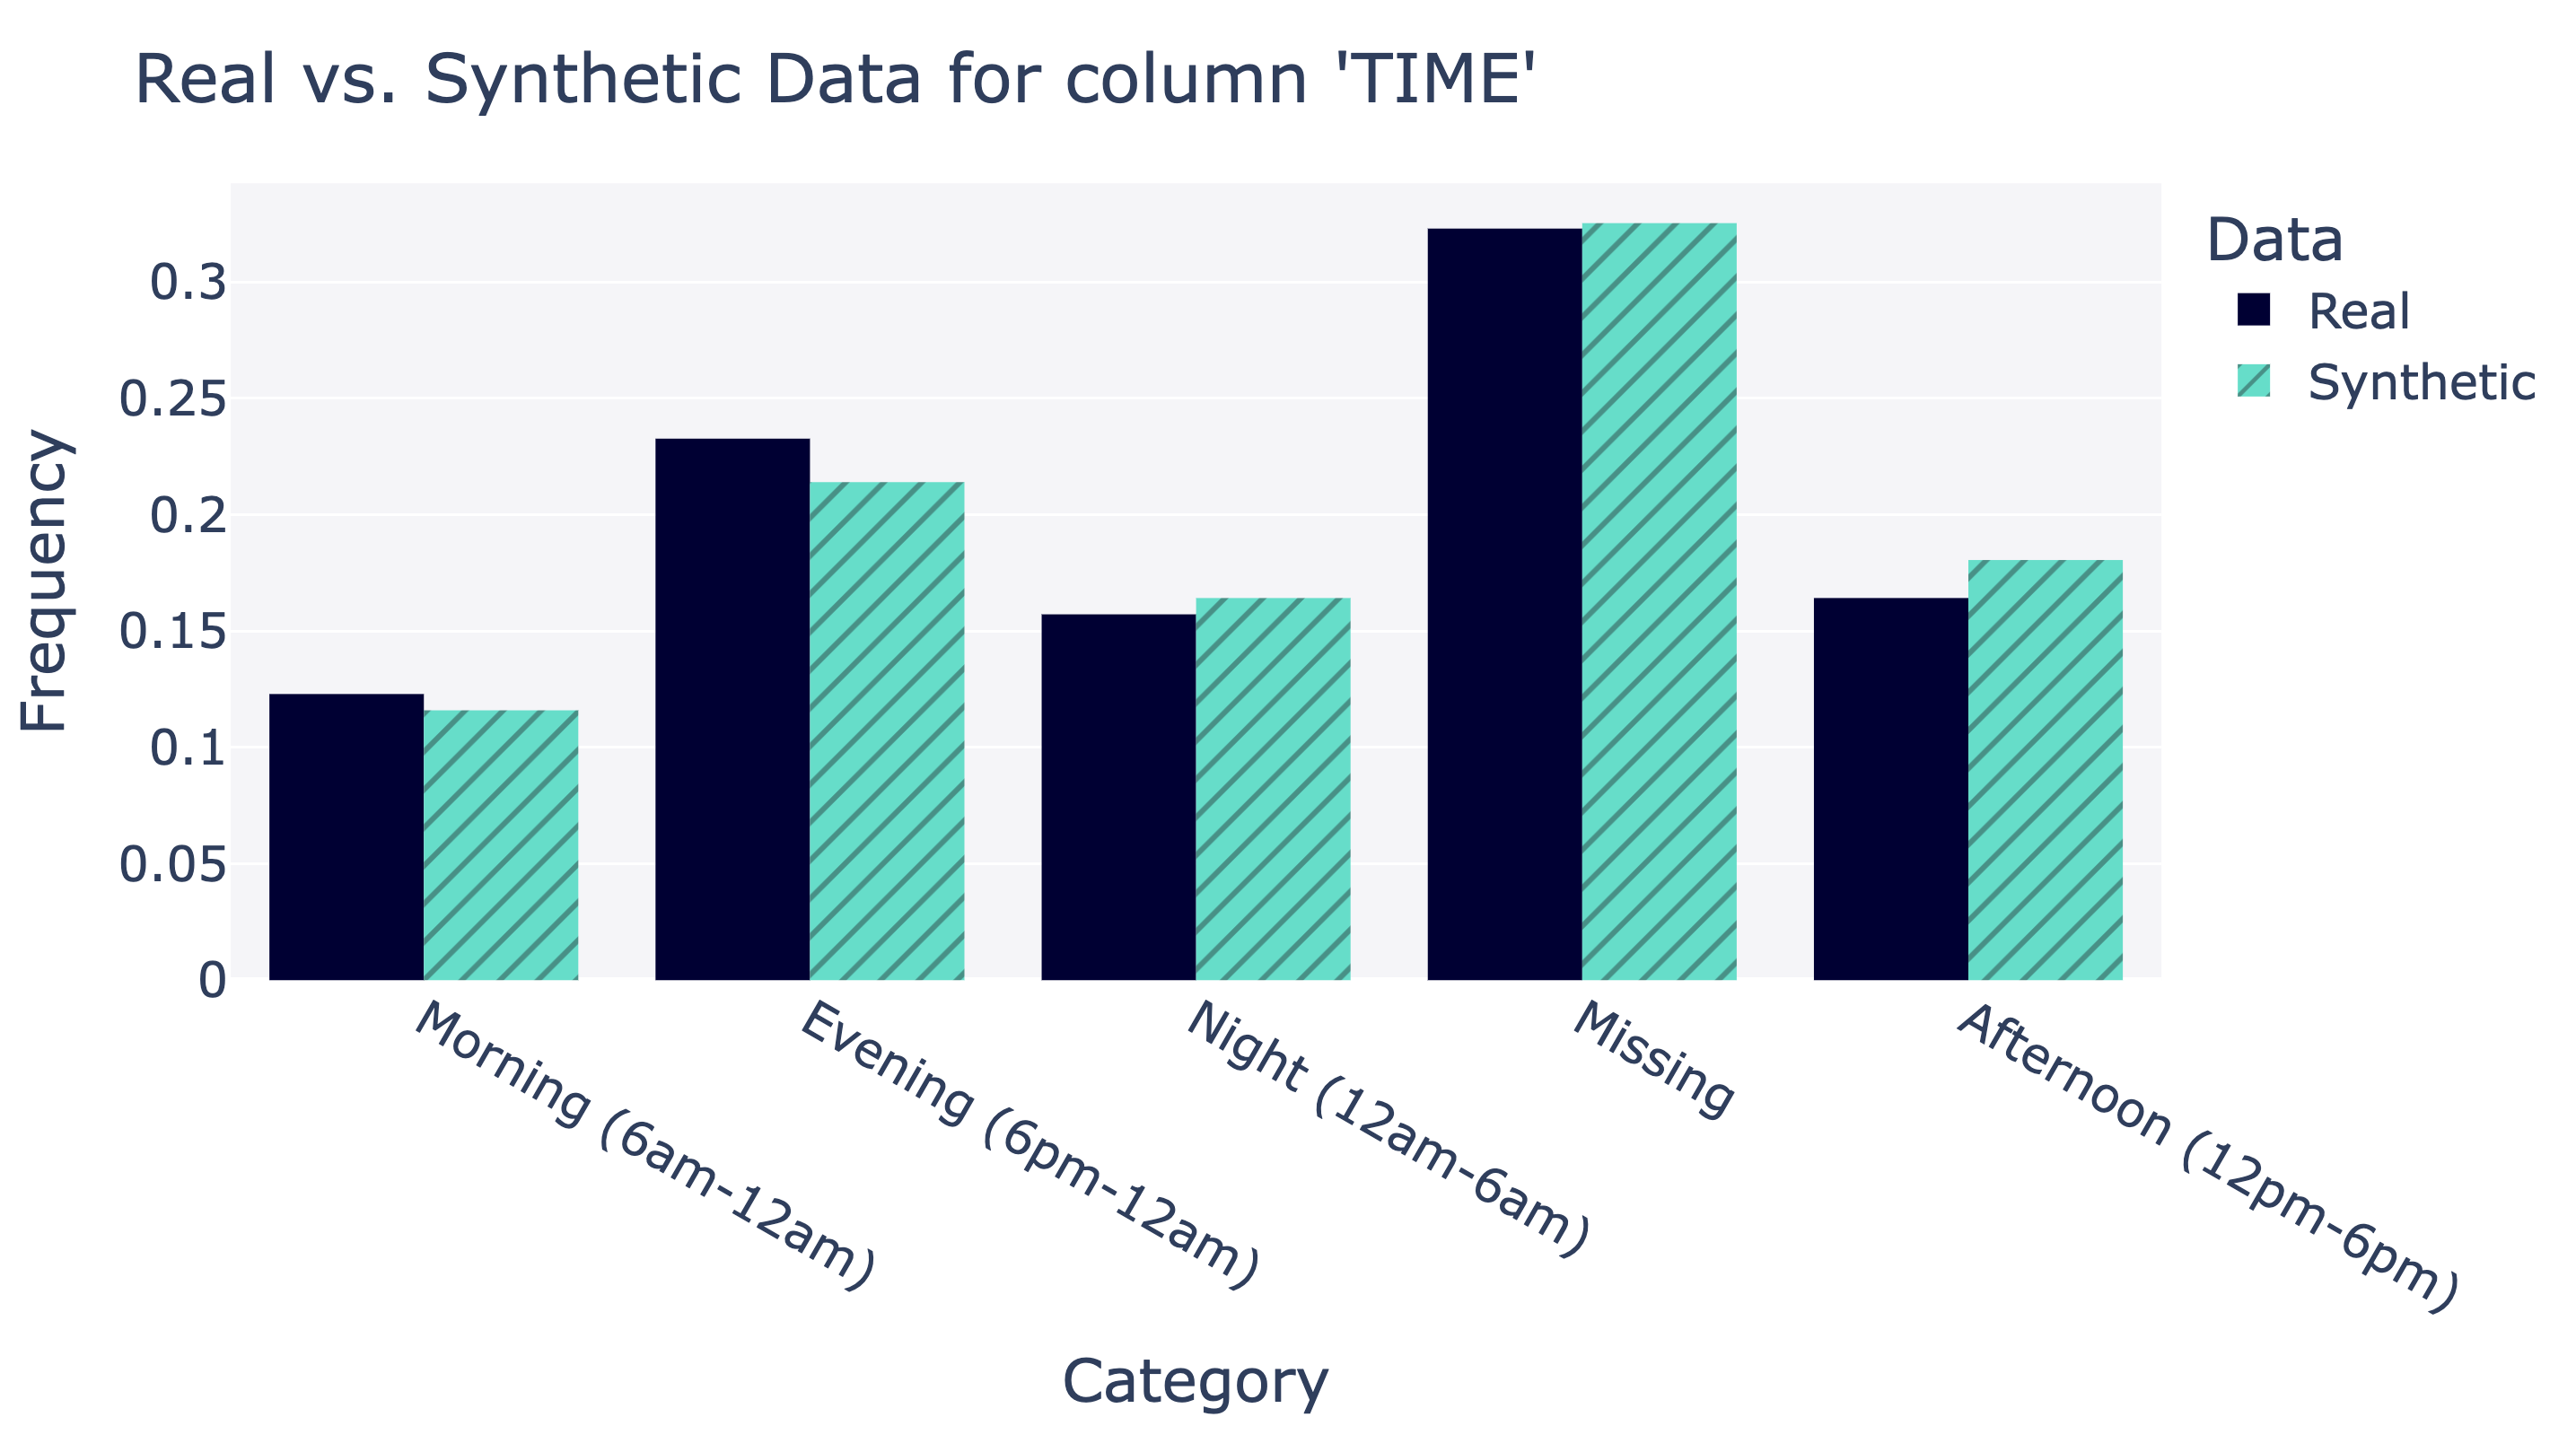
\includegraphics[width=0.8\textwidth]{Images/timefirst.png}
    \caption{Example of a synthesized variable with high quality score}
    \label{fig:proof_1}
\end{figure}
\vspace{10pt}

However, the univariate distribution in other variables, such as the judicial process, was significantly worse and below the desired threshold.

\vspace{10pt}
\begin{figure}[h!]
    \centering
    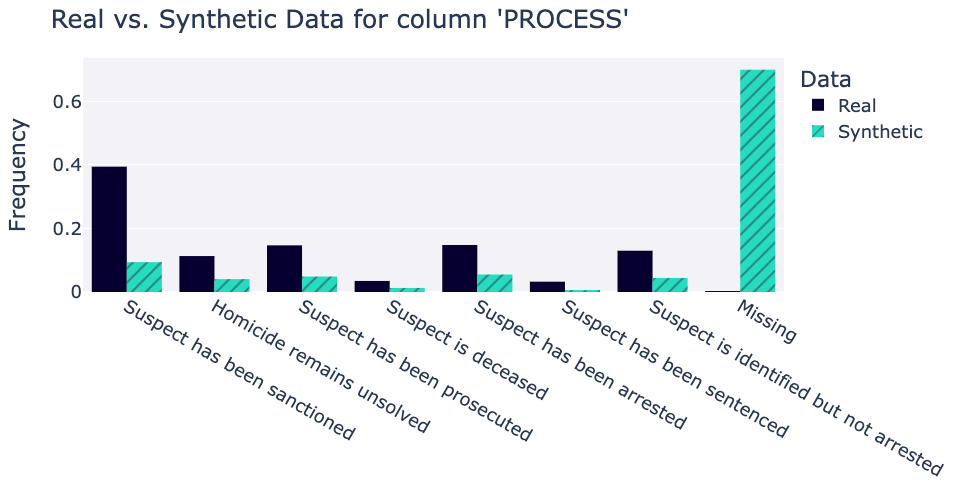
\includegraphics[width=0.8\textwidth]{Images/SENSYN_badsyn1.png}
    \caption{Example of a synthesized variable with low quality score}
    \label{fig:proof_1}
\end{figure}
\vspace{10pt}

Similarly, significant limitations are visible in the bivariate distributions, that is the relationship between variables.

\vspace{10pt}
\begin{figure}[h!]
    \centering
    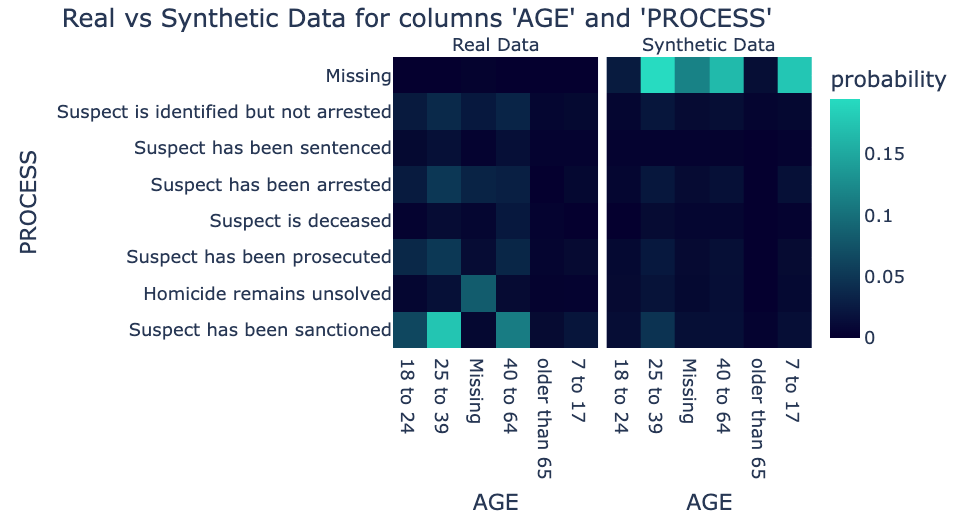
\includegraphics[width=0.8\textwidth]{Images/SENSYN_biva1.png}
    \caption{Example of bivariate relationship comparison across original and synthetic data}
    \label{fig:proof_1}
\end{figure}
\vspace{10pt}

Simply based on these limitations, we concluded that the synthetic dataset did match the requirements set out in the beginning. As such, we did not conduct further analysis, such as replication studies, or an evaluation of the privacy guarantees of the synthetic data.\\


\textbf{Reflections}

After deliberations, we determined two potential causes for the lower than expected quality of the synthetic dataset. First, our data is relatively complex as it spans over three tables, meaning that the synthesiser has to learn not only about the patterns and relationships within \textit{one} table (e.g. the relationship between the victim's gender and age) but also across the three tables (e.g. the relationship between type of crime scene, gender of the victim and gender of the perpetrator). In addition, the synthesiser has to replicate relatively many variables (29 divided over the three tables) and many categories within those variables. As mentioned previously, some of the variables have up to 35 categories, with each of these categories having certain patterns and relationships with all the other categories across all variables. Given that about 70 percent of the variables in the synthetic dataset compared well to the original dataset, but the remaining 30 percent did not, we believe that the synthesiser over-corrected, meaning that it tried to mimic as many patterns and relationships as best as possible at the costs of the quality of the patterns and relationships that remained. A second problem that might have impacted the results is that our dataset contains relatively little data, with 1271 cases, information on 1348 victims and 1711 perpetrators. Although this amount is technically sufficient to train a model on the patterns and relationships within that dataset, more data provides a better ground for detecting all underlying patterns and relationships, especially when the data contains many variables as in this case.

Therefore, we decided to address these causes in a second round, meaning that we started again at the step of data preparation. 


\subsection{Second attempt}

\textbf{Step 1: Preparations}\\
In order to address the possible causes of the limited data utility in the first attempt, we decided to \textbf{(a)} reduce the complexity of the data as much as possible, and \textbf{(b)} to increase the amount of original data.

To reduce the complexity of the data, we decided to minimise both the number of variables, as well as the number of categories within the variables. In total, we excluded six variables: the profession of the victim or perpetrator, whether the victim or perpetrator was under the influence of drugs or alcohol, whether the victim or perpetrator had a violent history, the main motive of the perpetrator and whether the perpetrator committed or attempted suicide. These variables had a vast amount of missing data (and therefore the lowest quality) and were deemed the least important by the project team members with expertise on homicide research. To reduce the number of categories within each variable, we first detected categories with only few cases, such as sexual homicides. After, we aimed to merge these categories together into categories of 'other', based on the number of cases, as well as on logical reasoning. For example, the Dutch Homicide Monitor differentiates between three different types of child homicides: infanticides - the killing of newborns -, the homicide of children by someone in the child's family and the killing of a child by someone outside of the child's family. For the sake of decreasing categories, these three types were merged into one category: \textit{child homicide}. Yet, in order to keep as much detail as possible in the original and thus also the synthetic data, we merged as little categories as deemed necessary at this stage in the process.

To increase the amount of original data through which the synthesiser can learn about the patterns and relationships, we decided to broaden the scope of homicide data included, from ten years of homicide data to twenty years of homicide data. As a result, the original dataset used to train the synthesiser now contained 3152 cases, and information on 3358 victims and 4394 perpetrators. \\

\textbf{Step 2: Choosing generation method and tool}\\
The generation method and chosen tool (Synthetic Data Vault) remained the same. However, given that we added new data and recoded some of our variables, we re-ran the steps for data cleaning and the preparation of the meta-data.

\begin{figure}[H]
    \centering
    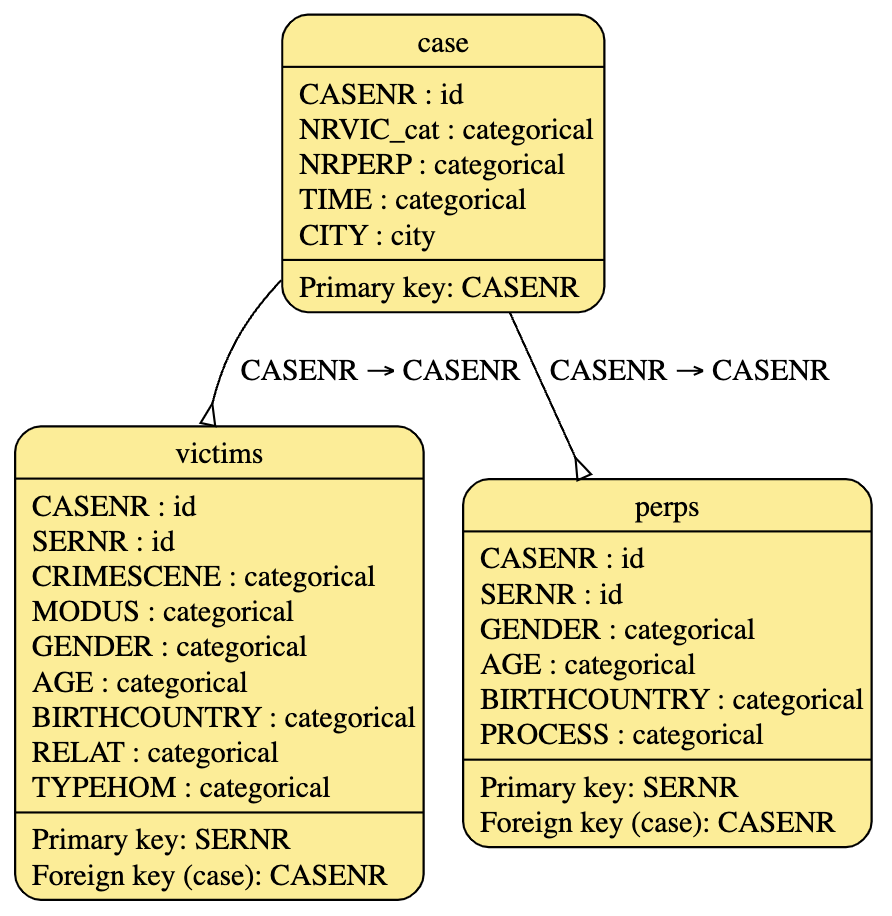
\includegraphics[width=0.8\textwidth]{Images/meta2.png}
    \caption{Dutch Homicide Monitor split into three separate datasets: cases, victims \& perpetrators}
    \label{fig:proof_1}
\end{figure}
\vspace{10pt}


\textbf{Step 3: Generation}\\
As in the previous attempt, we created a synthesiser based on the new meta-data and fed the synthesiser our new dataset to learn the patterns and relationships. Yet, considering that the new adaptions were made in the original dataset, the process remained the same.

\textbf{Step 4: Privacy and utility evaluation}\\
With regards to the utility of the data, we detected similar issues as during the first attempt. Again, most of the variables in the synthesised dataset compared well to the original dataset, yet other variables were synthesised poorly. The bivariate relationships of the variables improved compared to the first attempt, yet were still not at a quality that we were satisfied that this synthetic dataset fulfils the statistical requirements set in the beginning. \\

\vspace{10pt}
\begin{table}[H]
\small
\resizebox{\textwidth}{!}{
\begin{tabular}{@{}lll@{}}
\toprule
Quality Type &
  Score (\%) &
  Interpretation \\ \midrule
Data validity &
  100 &
  \begin{tabular}[c]{@{}l@{}}The synthetic data has the same internal structure \\ as the original one\end{tabular} \\
Data structure &
  100 &
  \begin{tabular}[c]{@{}l@{}}The synthetic data has the same columns \\ with the same names\end{tabular} \\
Relationship validity &
  99.99 &
  \begin{tabular}[c]{@{}l@{}}Each case in the victim \& perpetrator datasets \\ are linked to a case in the case dataset\end{tabular} \\
Univariate distribution &
  75.84 &
  \begin{tabular}[c]{@{}l@{}}A variable in the synthetic dataset is on average \\ 75\% similar to the variable in the real dataset\end{tabular} \\
Bivariate distribution within one table &
  51.51 &
  \begin{tabular}[c]{@{}l@{}}The relationship between two variables in the \\ synthetic data is about 50\% similar to the \\ relationship in the real dataset\end{tabular} \\
Structure across tables &
  90.97 &
  \begin{tabular}[c]{@{}l@{}}Around 90\% of cases in the synthetic dataset has the \\ same number of victims and perpetrators associated \\ as in the real dataset\end{tabular} \\
Bivariate distribution across tables &
  63.9 &
  \begin{tabular}[c]{@{}l@{}}The relationship between two variables across \\ the three synthetic datasets is about 64\% similar \\ to the relationship in the real data\end{tabular} \\
Overall &
  70.56 &
  \begin{tabular}[c]{@{}l@{}}Overall, the synthetic dataset compares \\ around 70\% to the real data\end{tabular} \\ \bottomrule
\end{tabular}
}
\caption{General quality report}
\label{tab:my-table}
\end{table}
\vspace{10pt}

\begin{table}[H]
\centering
\small
\begin{tabular}{@{}ll@{}}
\toprule
Variable                                              & Score (\%)   \\ \midrule
Perpetrator birth country                             & 89.87 \\
Status of case against perpetrator in judicial system & 82.36 \\
Perpetrator age                                       & 75.78 \\
Perpetrator gender                                    & 30.5 \\ \bottomrule
\end{tabular}
\caption{Example: quality of each variable in the synthetic perpetrator dataset, ranked from highest to lowest similarity score}
\label{tab:my-table}
\end{table}
\vspace{10pt}


\begin{figure}[H]
\centering
    \hfill
    \subfigure[Example of a synthesised variable with high quality score]{
        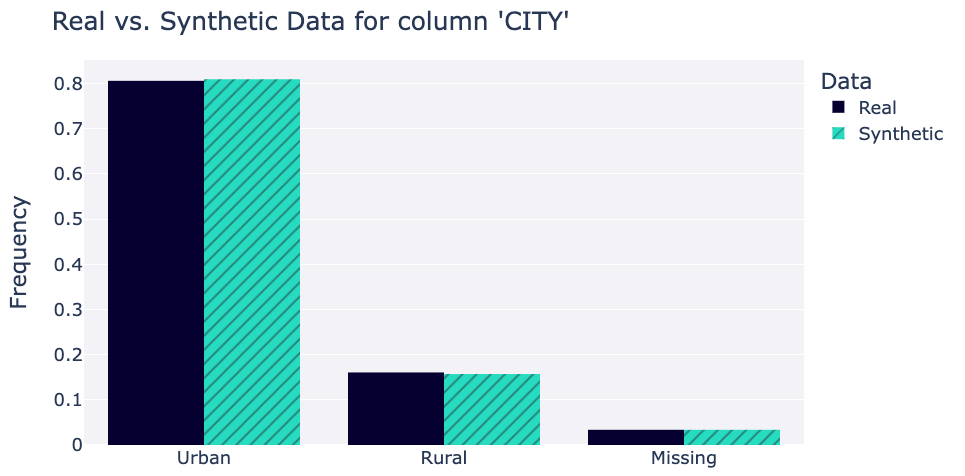
\includegraphics[width=0.8\textwidth]{Images/SENSYN_good2.png}
        \label{fig:subfig2}
    }
    \hfill
    \subfigure[Example of a synthesised variable with low quality score]{
        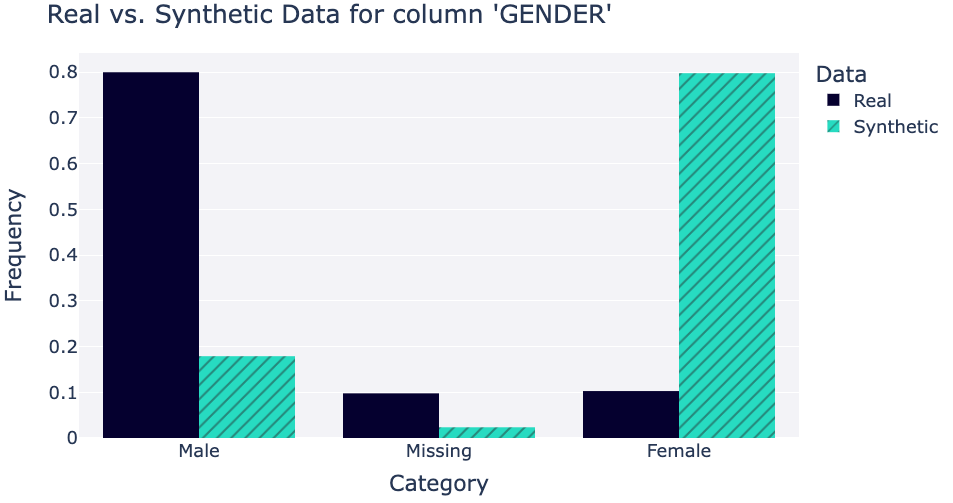
\includegraphics[width=0.8\textwidth]{Images/SENSYN_bad2.png}
        \label{fig:subfig2}
    } 
    \hfill
    \subfigure[Example of bivariate relationship comparison across original and synthetic data]{
        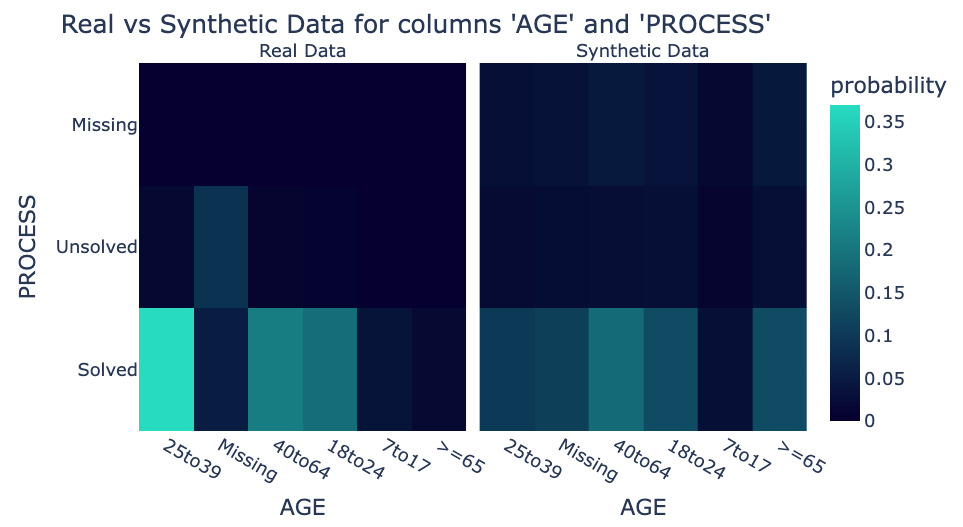
\includegraphics[width=0.8\textwidth]{Images/SENSYN_biva2.png}
        \label{fig:subfig2}
    }
    \caption{Quality of the second synthetic version of the DHM (continued)}
    \label{fig:main_fig}
\end{figure}


Again, we did not conduct any privacy analyses due to the low level of utility.\\

\textbf{Reflections}

Going back to the potential causes of the limited quality, we concluded that the increased amount of data had little impact on the quality of the synthetic dataset. Instead, we had to again review how to reduce the complexity in our data.

Initially, we followed the same procedure as in our previous attempt, by merging categories within variables wherever logically possible. For example, the variable on victim-perpetrator relationship went from 35 categories to only ten categories.

Unfortunately, although the quality of the synthetic dataset improved slightly with each merging, it did not reach a level of quality that was satisfying. Moreover, at a certain point, even further merging of the variables would have significantly changed the level of detail in the dataset, which is one of the main advantages of the original Dutch Homicide Monitor.

\subsection{Final attempt}

\textbf{Step 1: Preparations}\\
With this conclusion in mind, we decided to reduce the complexity, by reducing the multi-table approach to a single-table approach in which the synthesiser only has to recognise the patterns and relationships across one table instead of three. This meant that we had to merge the three tables with the original data (case table, victim table and perpetrator table) back into one single table. With the original structure, the synthesiser would be able to learn the dependencies across the rows, thus individuals that are involved as either victim or perpetrator in the same case. As such, we had to concede that we would not be able to create a synthetic dataset that would allow analysis on the level of case, victim \textbf{and} perpetrator. Based on domain expertise, we decided to merge the information of the main perpetrator onto the row of each associated victim and add a variable that would define one main victim per case. As a result, all information on each individual case and each individual victim is kept in the dataset, yet information for some perpetrators (specifically in cases with multiple perpetrators) were lost. In addition, to increase the quality of the remaining data, we decided to again only use homicide data of ten years as this is the most complete data in the original dataset. Finally, we also reverted most of the merging of categories within the variables, in order to keep as much detail as possible.

\textbf{Step 2: Choosing generation method and tool}] \\
Given the changed structure of the original dataset, we had to revisit the requirements of the Synthetic Data Vault for single table synthesis. In essence, only few changes had to be made, in particular with regards to the meta-data.

\vspace{10pt}
\begin{figure}[H]
    \centering  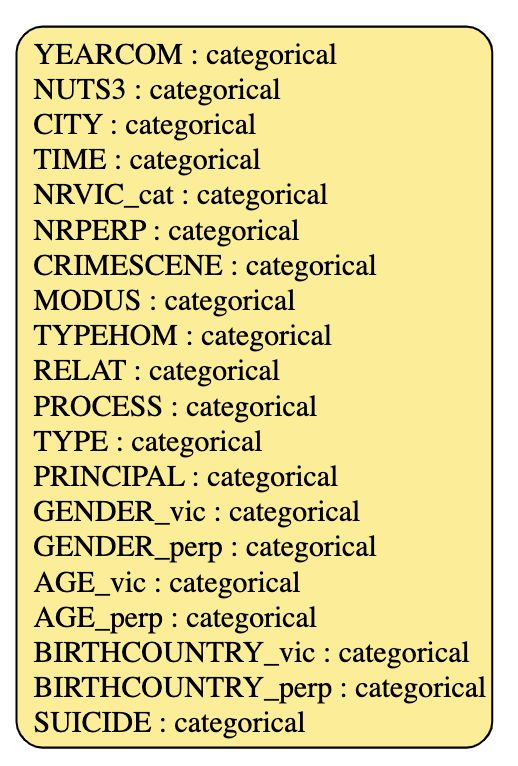
\includegraphics[width=0.5\textwidth]{Images/meta3.png}
    \caption{Dutch Homicide Monitor as one dataset, with each row representing one victim}
    \label{fig:proof_1}
\end{figure}
\vspace{10pt}

\textbf{Step 3: Generation} \\
As in the previous steps, we used the meta-data of the single table with homicide information to create a synthesiser, and trained said synthesiser with the original dataset.

\vspace{10pt}
\begin{lstlisting}[caption={Synthetic Data Generation: Final Attempt}, label={lst:gen_first}]
from sdv.single_table import GaussianCopulaSynthesizer

synthesizer = GaussianCopulaSynthesizer(metadata,
                                        locales=['nl_NL']

synthesizer.add_constraints([IPHConstraint,kindermoordConstraint])

synthesizer.fit(DHM)
synthetic=synthesizer.sample(num_rows=1364)
\end{lstlisting}
\vspace{10pt}

\textbf{Step 4: Privacy and Utility Evaluation}

In this attempt, both the comparison of the univariate as well as bivariate patterns between the original and synthetic data looked significantly improved, which is supported by the quality report provided by the Synthetic Data Vault package.

\vspace{10pt}
\begin{table}[H]
\small
\resizebox{\textwidth}{!}{
\begin{tabular}{@{}lll@{}}
\toprule
Quality Type &
  Score (\%) &
  Interpretation \\ \midrule
Data validity &
  100 &
  \begin{tabular}[c]{@{}l@{}}The synthetic data has the same internal structure \\ as the original one\end{tabular} \\
Data structure &
  100 &
  \begin{tabular}[c]{@{}l@{}}The synthetic data has the same columns \\ with the same names\end{tabular} \\
Univariate distribution &
  97.8 &
  \begin{tabular}[c]{@{}l@{}}A variable in the synthetic dataset is on average \\ 98\% similar to the variable in the real dataset\end{tabular} \\
Bivariate distribution within one table &
  89.67 &
  \begin{tabular}[c]{@{}l@{}}The relationship between two variables in the \\ synthetic data is about 90\% similar to the \\ relationship in the real dataset\end{tabular} \\
Overall &
  93.74 &
  \begin{tabular}[c]{@{}l@{}}Overall, the synthetic dataset compares \\ around 94\% to the real data\end{tabular} \\ \bottomrule
\end{tabular}
}
\caption{General quality report}
\label{tab:my-table}
\end{table}
\vspace{10pt}

\begin{table}[H]
\centering
\small
\begin{tabular}{@{}ll@{}}
\toprule
Variable                                              & Score (\%)   \\ \midrule
Type: victim or perpetrator?                          & 99.93 \\
City homicide was committed in                        & 99.79 \\
Number of perpetrators                                & 99.21 \\
Status of case against perpetrator in judicial system & 99.13 \\
Number of victims                                     & 98.98 \\
Time of day homicide was committed                    & 98.87 \\
Perpetrator gender                                    & 98.81 \\
Perpetrator birthcountry                              & 98.3  \\
Type of crimescene                                    & 98.04 \\
Victim gender                                         & 97.9  \\
Victim age                                            & 97.38 \\
Perpetrator age                                       & 97.32 \\
Modus operandi                                        & 97.11 \\
Victim-perpetrator relationship                       & 96.95 \\
Victim birthcountry                                   & 96.89 \\
Year homicide was committed                           & 95.2  \\ 
Region homicide was committed                         & 94.92 \\
Context of homicide                                   & 93.53 \\ \bottomrule
\end{tabular}
\caption{Quality of each variable in the synthetic dataset, ranked from highest to lowest similarity score}
\label{tab:my-table}
\end{table}

\begin{figure}[H]
    \hfill
    \subfigure[Example of a synthesised variable with high quality score]{
        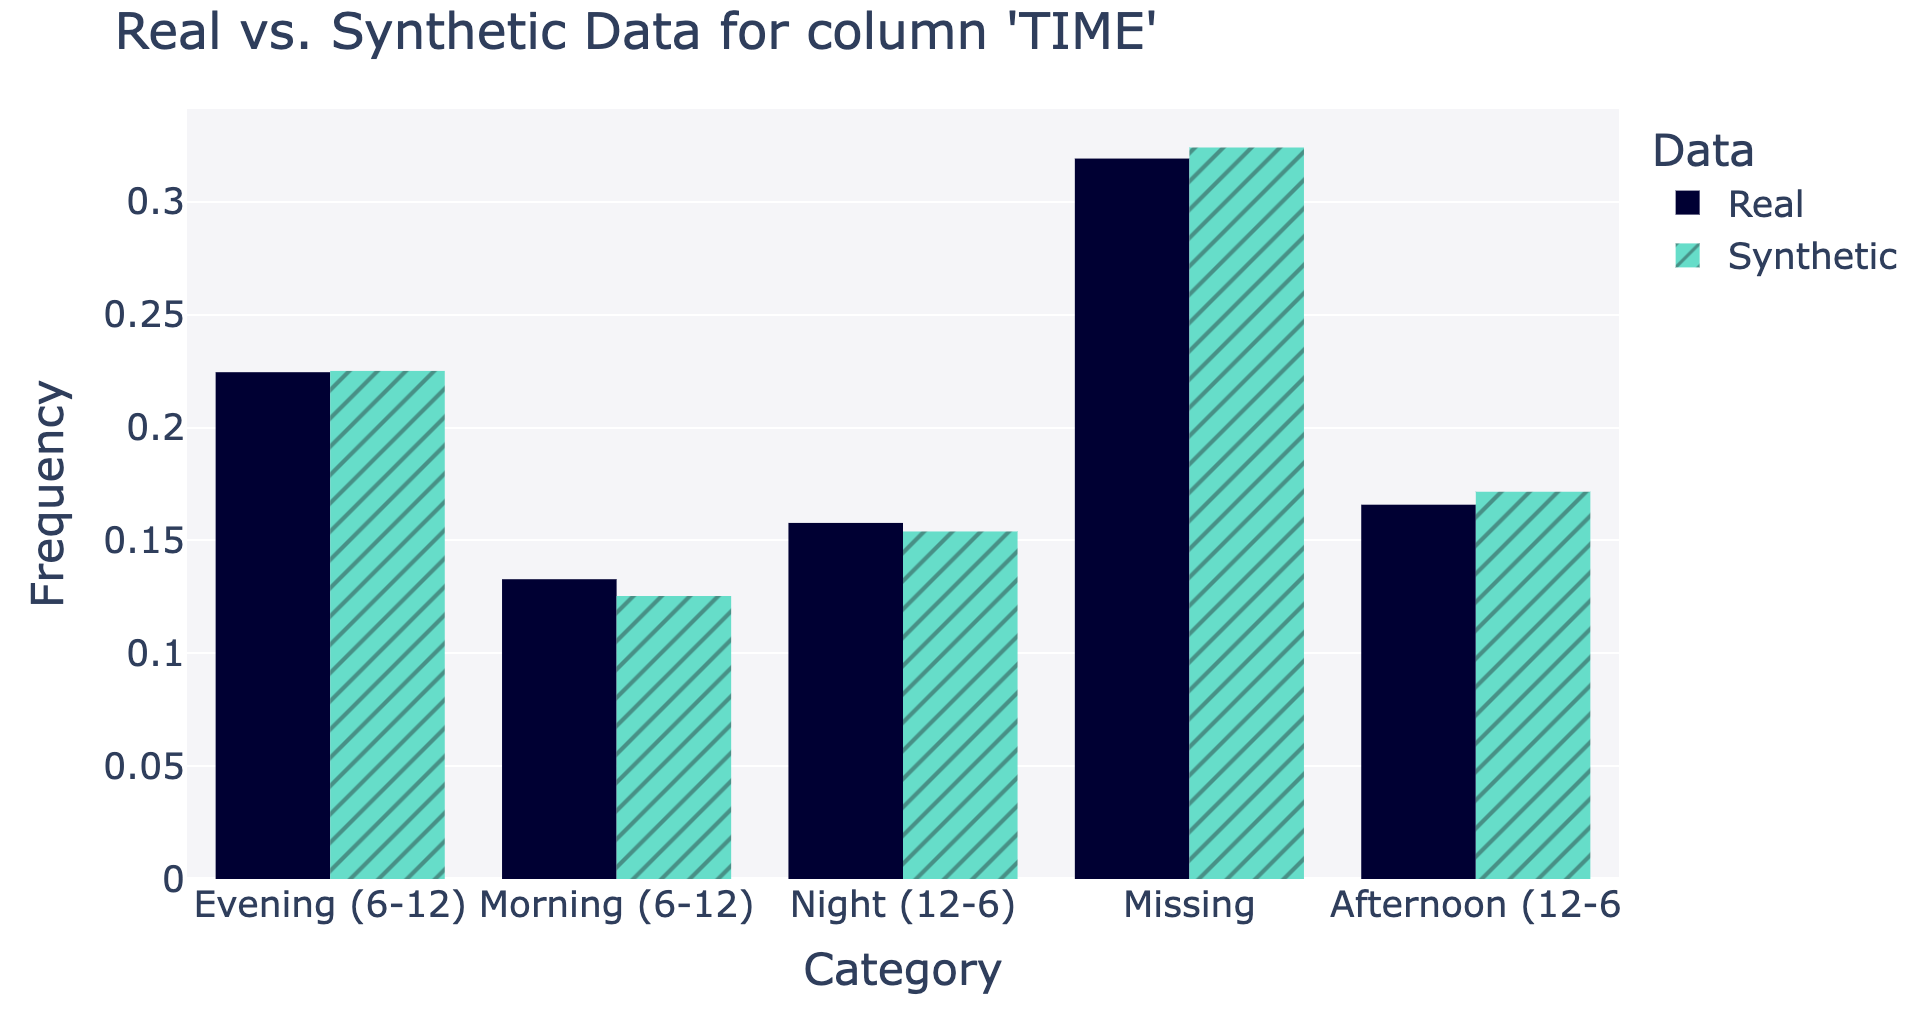
\includegraphics[width=0.8\textwidth]{Images/SENSYN_goodFINAL.png}
        \label{fig:subfig2}
    }
    \hfill
    \subfigure[Example of a synthesised variable with the lowest quality score]{
        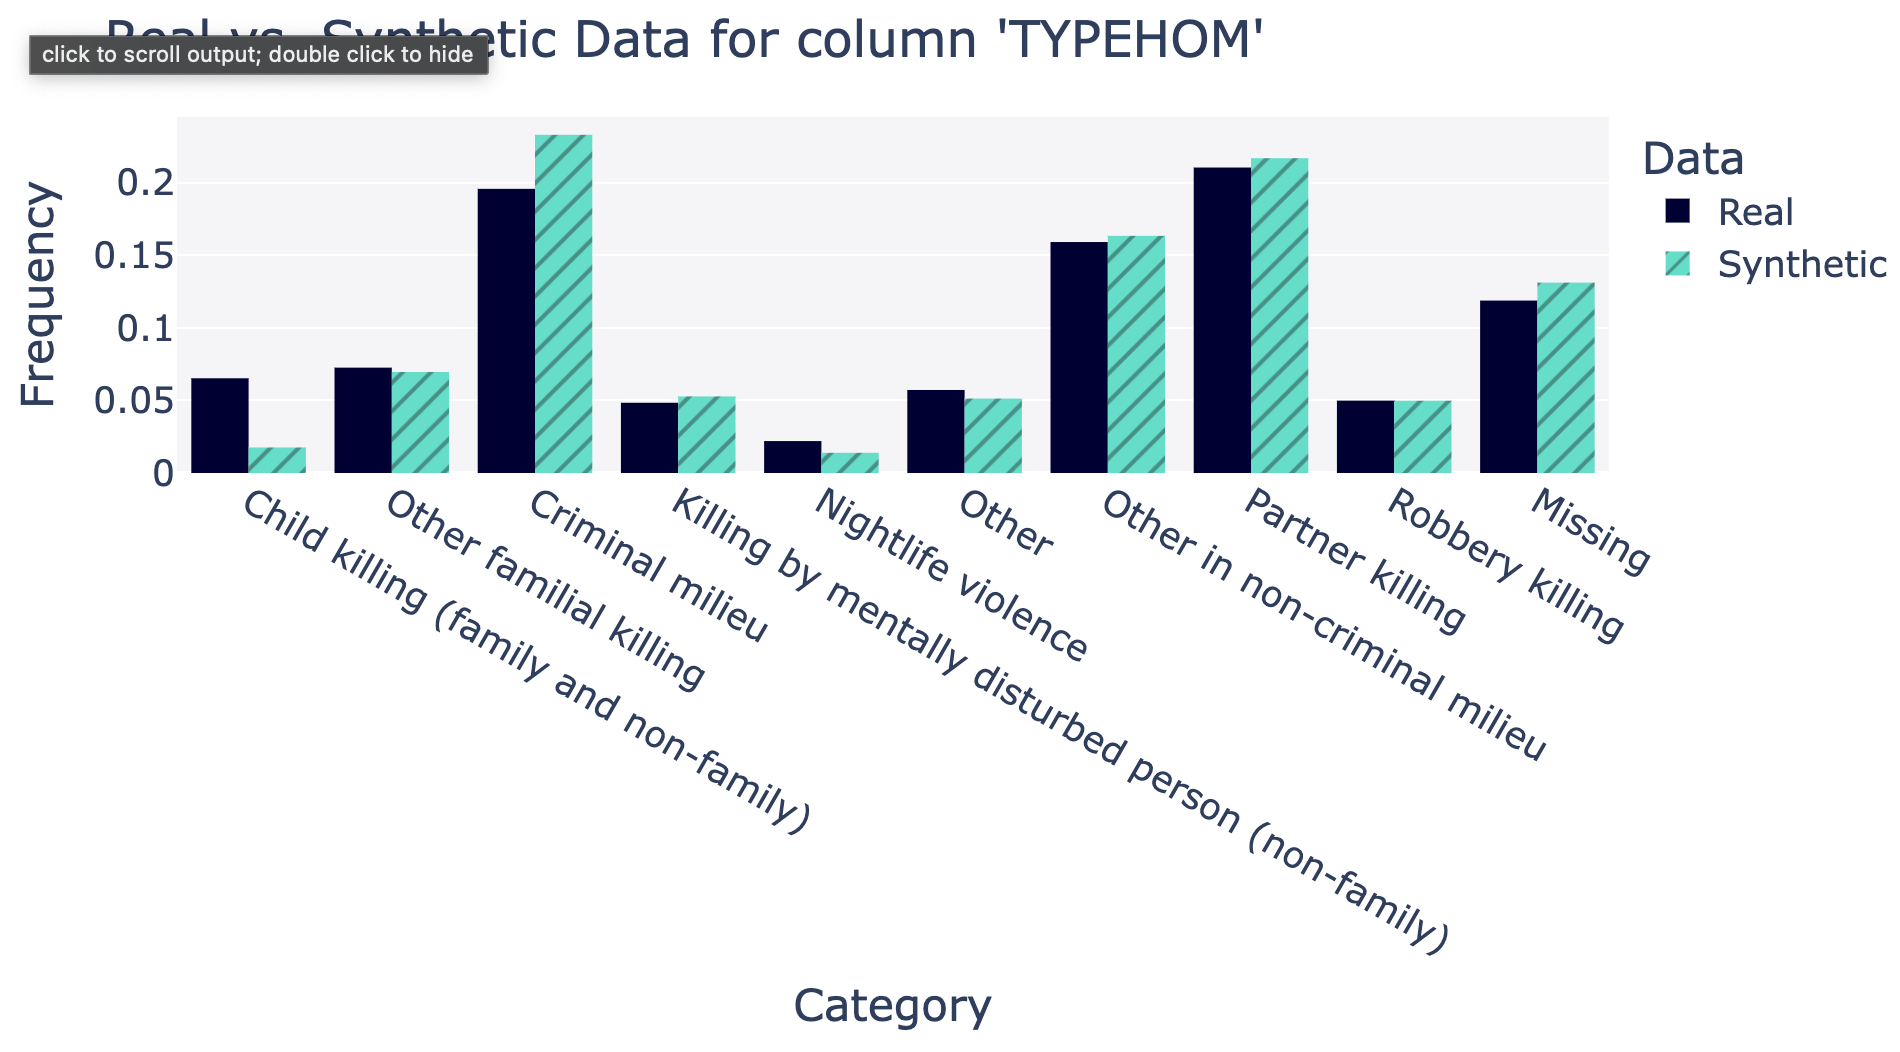
\includegraphics[width=0.8\textwidth]{Images/SENSYN_badFINAL.png}
        \label{fig:subfig2}
    }
    \centering
    \hfill
    \subfigure[Example of bivariate relationship comparison across original and synthetic data]{
        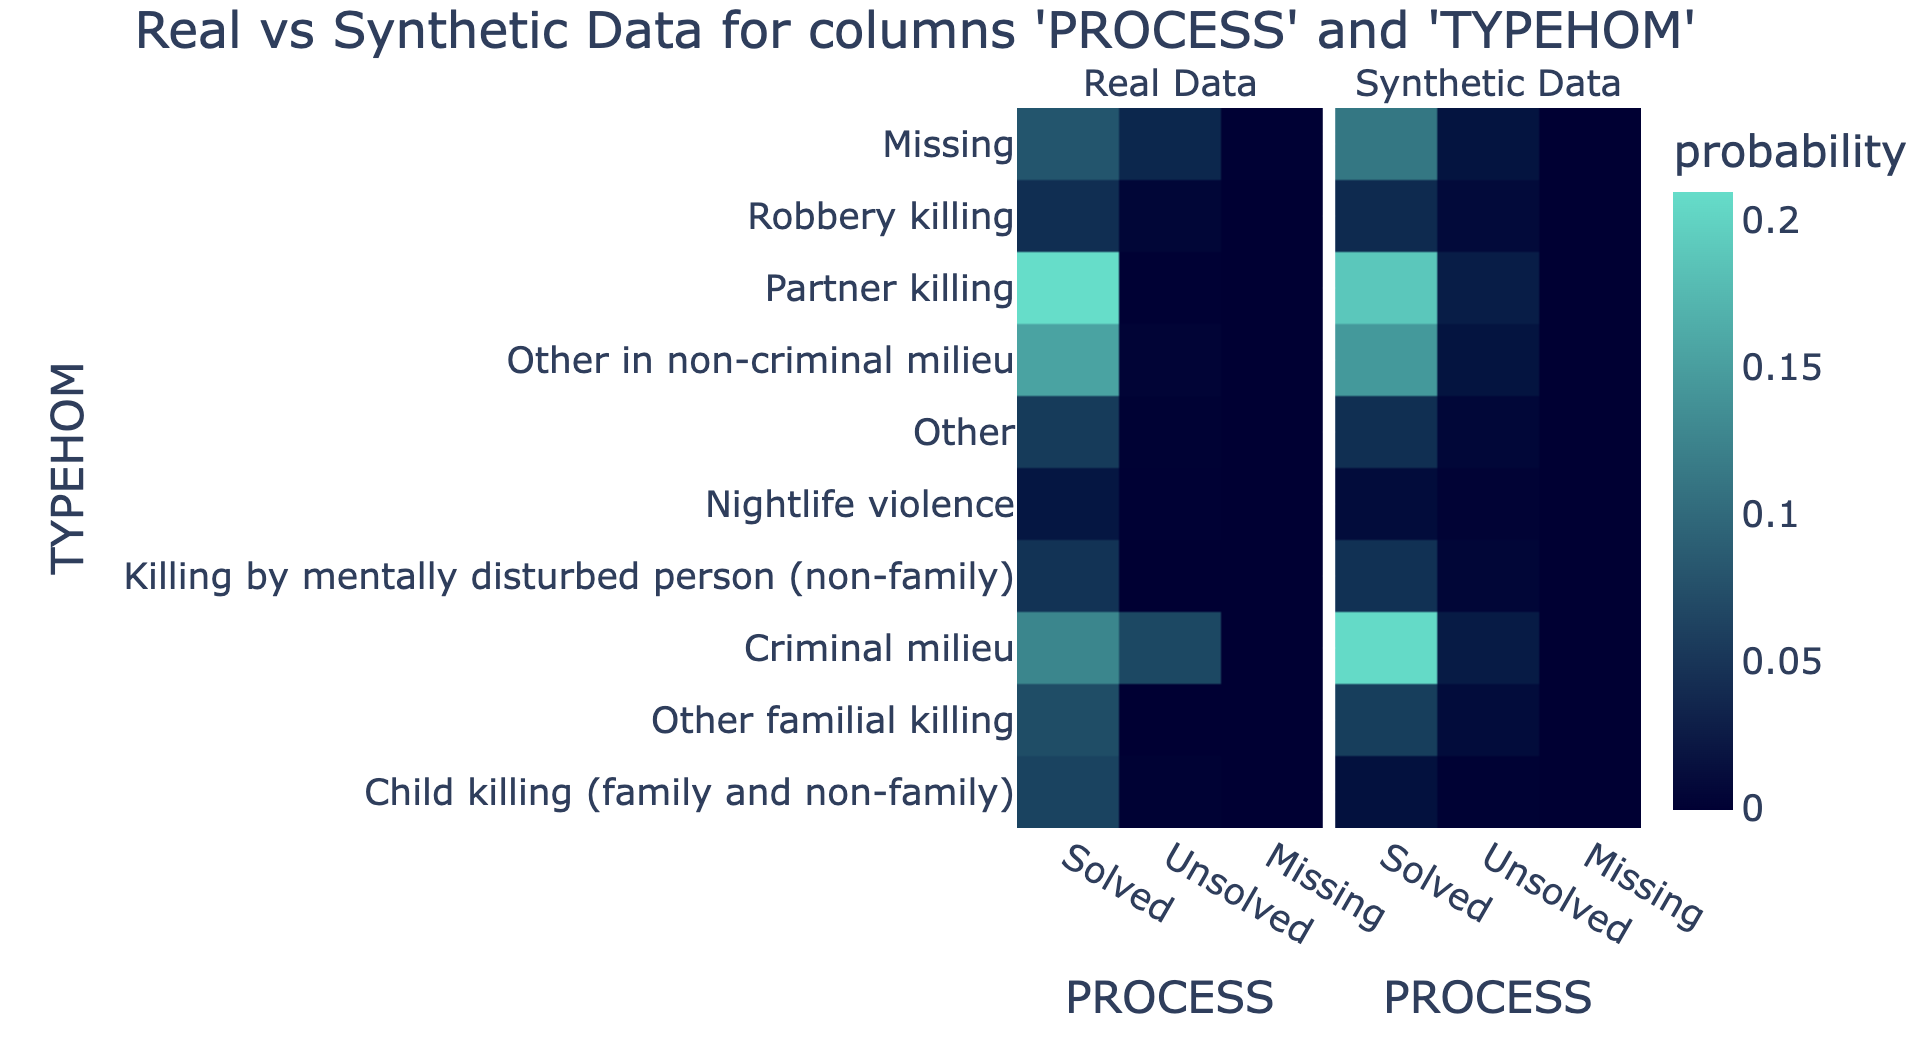
\includegraphics[width=0.8\textwidth]{Images/SENSYN_bivaFINAL.png}
        \label{fig:subfig2}
    }
    \caption{Quality of the final synthetic version of the DHM (continued)}
    \label{fig:main_fig}
\end{figure}
\clearpage


Overall, this synthetic version of the Dutch Homicide Monitor satisfied our requirements with regards to data utility.

With regards to data privacy, we conducted several tests to check whether the safeguarding of sensitive and personal data is equally satisfying. First, we randomly selected about twenty cases from the original dataset and tried to identify cases that match their profiles in the synthetic dataset. In addition, we identified certain outliers in the original dataset, e.g. individuals with unusual combination of attributes, and tested whether we were able to identify similar cases in the synthetic dataset.
In both cases, were not able to detect one-on-one matches between the original and synthetic dataset with our chosen sample and outliers. Finally, we used privacy-metrics included in the SDV-package, the so-called \textit{Privacy Against Inference} metrics. These metrics calculate the risk of an attacker learning sensitive information based on the synthetic dataset, assuming that the attacker already has some information based on real data. The metrics allow for a simulation of this risk with all possible variable combinations.

\vspace{10pt}
\begin{lstlisting}[caption={SDV privacy metrics example}, label={lst:gen_first}]
from sdmetrics.single_table import CategoricalKNN,CategoricalRF

CategoricalKNN.compute(
    real_data=case,
    synthetic_data=synthetic,
    key_fields=['GENDER_vic','CRIMESCENE'], #these are the variables we assume the attacker already knows
    sensitive_fields=['RELAT'] #this is the variable the attacker wants to know
\end{lstlisting}
\vspace{10pt}

For each variable-combination, the algorithm provides a percentage; 0\% means that the data is not safe at all, 100\% means that the data is completely safe. In the example in the listing above, the information about the victim-perpetrator relationship was 79.7\% safe, given that the attacker already knows the victim's gender and the type of crimescene.

%%%%%%%%%%%%%%%%%%%%%%%%%%%%%%%%%%%%%%%%

\section{Concluding reflections}

\subsection{The process}
Taking into account data preparation and necessary adaptions for each cycle, the overall process only took about two full days; the actual generation of the synthetic data between a few seconds for final single table to a few minutes for the most complex multi-table. Data preparation and cleaning took most of the time. Moreover, through the detailed documentation provided by the Synthetic Data Vault library, as well as a helpful community of users online, any questions or problems along the process have quickly been answered or solved. In addition, the synthesis of data with the use of the Synthetic Data Vault has proven very accessible, even for someone without extensive knowledge of programming or synthetic data. 

\subsection{The data}
In the beginning of the process, we set high aims and requirements for the synthetic version of the Dutch Homicide Monitor. In simple terms, we wanted to create a synthetic dataset that mimics the original data enough to be used for advanced scientific analysis, to be informative for non-scientific purposes but to safeguard the privacy of all individuals included in the dataset. In the end, not all of the requirements have been met, in particular the requirement that the full original dataset had to be synthesised. Due to the complexity of the original data impacting the quality of the synthetic data, we had to opt to exclude information on certain perpetrators (in cases in which there were more than one perpetrator). Thus, information from the original dataset was lost during the process. The final synthetic dataset, however, provides a good balance between privacy assurance and data quality for the intended use of creating a dataset that can be displayed and provides detailed information about the phenomenon of homicide in the Netherlands. Here, it should be noted that the usefulness of the dataset is context- and use-case dependent, meaning that the dataset may be less useful for other tasks, such as replication specific studies focusing on homicide perpetration or predictive tasks.

\subsection{Open \& FAIR data}
With regards to open science principles, the synthetic dataset has been developed with the FAIR principles in mind. Therefore, the full disaggregated data can be found, used and downloaded at the \href{https://www.dutchhomicide.streamlit.io}{projects webpage}. In addition, the \href{https://github.com/KKrusselmann/SENSYN}{project's github page} includes meta data and codes used for the synthesis. 







\chapter{Conclusion: enhancing open science practices through synthetic data}
%%%%%%%%%%%%%%%%%%%%%%%%%%%%%%%%%%%%%%%%
% Chapter 6: Conclusion
%%%%%%%%%%%%%%%%%%%%%%%%%%%%%%%%%%%%%%%%

\label{conclusion}

Strict regulations surrounding personal and other sensitive data can seem at odds with the implementation of Open Science principles, creating hinderances for researchers, research support and other stakeholders. Synthetic data carries a lot of promises for enhancing data sharing practices, open datasets and the implementation of FAIR principles, in particular for sensitive data. It allows for the creation of artificial datasets that mimic real-world data whilst protecting private and personal information. These datasets can be shared, registered, fit to other open science standards and be used without many restrictions. So far, synthetic data is mostly discussed amongst data scientists, who develop new measures of utility and privacy, new computations for syntheses processes and advance already existing approaches. However, synthetic data is not applied much in research that does not focus on synthetic data as the topic of research yet. With fast developments in artificial intelligence and data science, synthetic data promises to become more and more useful in the future.  \\

We hope this guidebook provides a short introduction to the ideas and implementation of synthetic data, as well as practical tips on how synthetic data can be applied in everyday research to make it more open, findable, interoperable, accessible, and reusable.  




%%%%%%%%%%%%%%%%%%%%%%%%%%%%%%%%%%%%%%%%
% Appendix

\chapter{Appendix: Resources}
%%%%%%%%%%%%%%%%%%%%%%%%%%%%%%%%%%%%%%%%
% Chapter 7: Resources
%%%%%%%%%%%%%%%%%%%%%%%%%%%%%%%%%%%%%%%%

\label{resources}

\section{Resources on Open Science}
\section{Resources on Open Data and Personal Data}
\section{Resources on synthetic data}


%%%%%%%%%%%%%%%%%%%%%%%%%%%%%%%%%%%%%%%%
% Bibliography
\printbibliography

%%%%%%%%%%%%%%%%%%%%%%%%%%%%%%%%%%%%%%%%
% END MAIN DOCUMENT
%%%%%%%%%%%%%%%%%%%%%%%%%%%%%%%%%%%%%%%%

\end{document}  